\documentclass{beamer}
\usepackage{bookmark}
\usepackage{graphicx}
\usetheme[sectionpage=progressbar]{metropolis}           % Use metropolis theme
\title{Topological Data Analysis with Mapper: an Implementation in Cytoscape and an Application to Aptamers}
\date{August 29, 2024}
\author{George Clare Kennedy}
\institute{University of Iowa}

\AtBeginSection[]
{
\setbeamerfont{currentsection in toc}{size=\Large}
\begin{frame}{Section Map (!)}
  \tableofcontents[currentsection,sectionstyle=show/shaded,subsectionstyle=show/hide/hide,subsubsectionstyle=show/hide/hide/hide]
\end{frame}
}
\begin{document}
\begin{frame}
  \titlepage
\end{frame}
\begin{frame}{Outline}
  \tableofcontents[hideallsubsections]
\end{frame}

\section{Why TDA?}

\begin{frame}{Data is Big}
  \begin{itemize}
    \item Modern techniques allow for rich data collection and storage
    \item Size of datasets can be enormous in both observations (rows) and variables (columns)
  \end{itemize}
  \only<1>{
  \begin{figure}
    \begin{center}
      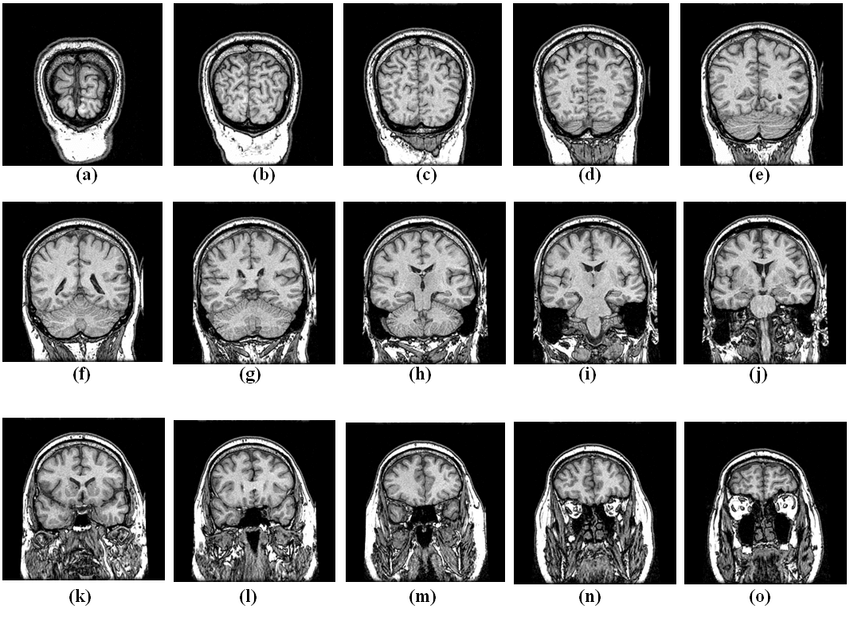
\includegraphics[width=.8\textwidth]{brains.png}
    \end{center}
  \end{figure}
  }
  \only<2>{
    \begin{figure}
      \begin{center}
        \includegraphics[width=.8\textwidth]{weatherstation.png}
      \end{center}
    \end{figure}
  }
\end{frame}

\begin{frame}{Geometry is Hard}
  \begin{itemize}
    \item High-dimensional space is extremely unintuitive
    \item If $V_n(r)$ is the volume of the $n$-dimensional ball with radius $r$, then for any $\varepsilon>0$, $$\lim_{n\to\infty}\frac{V_n(1-\varepsilon)}{V_n(1)}=0$$ i.e., the volume of balls lives almost entirely at the boundary
    \item Trying to analyze many characteristics creates combinatorial problems ($n!$ is big!)
  \end{itemize}
  
\end{frame}

\begin{frame}{Toning It Down}
  \begin{itemize}
    \item Broad idea: high dimensions $\implies$ low dimensions
    \item More specific idea: build a simplicial complex
    \item Simpler idea: build a 1-dimensional simplicial complex (that is, a graph)
    \item Enter: the Mapper algorithm (Singh et al, 2007)
    \vspace*{.5cm}
  \begin{figure}
    \begin{center}
      \hspace*{-1cm}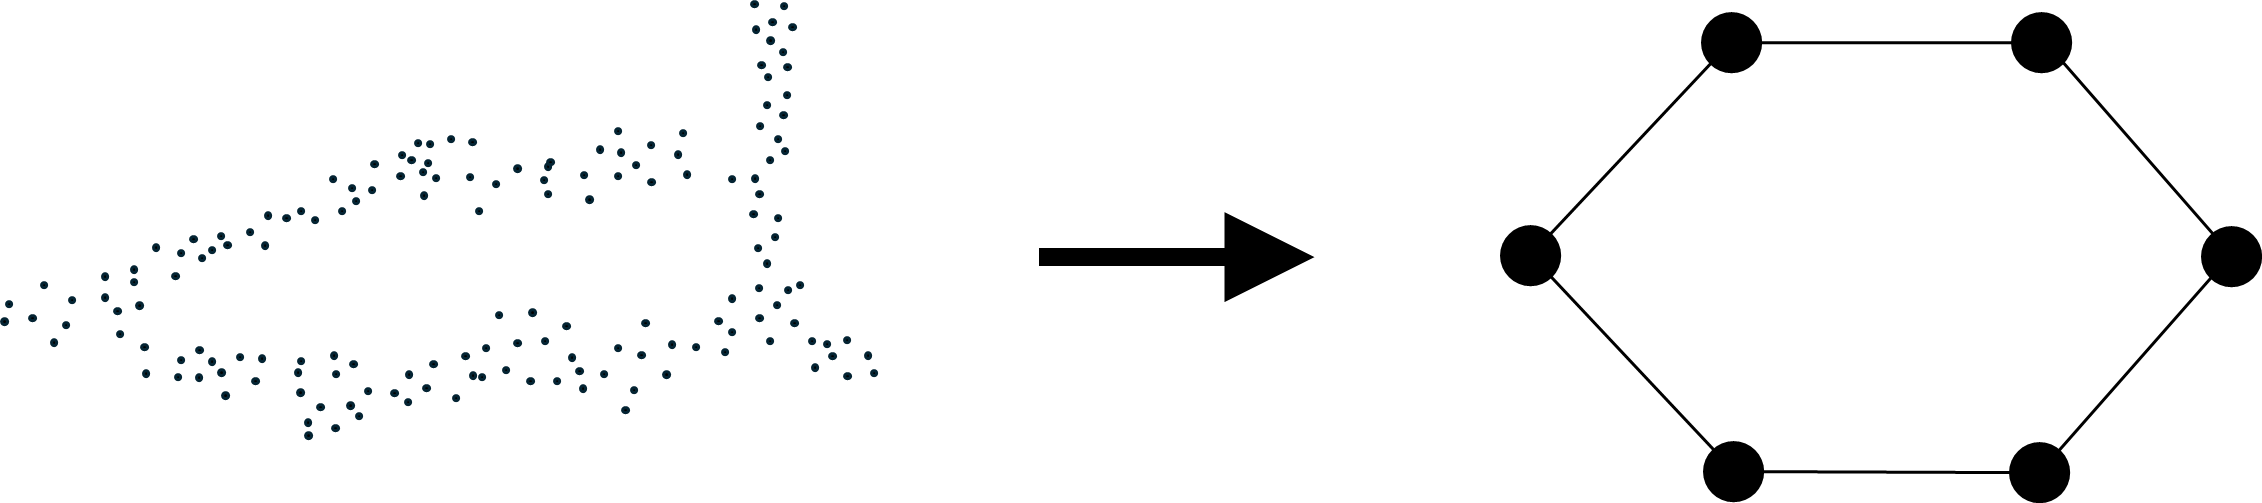
\includegraphics[width=1\textwidth]{datatograph.png}
    \end{center}
  \end{figure}
  \end{itemize}
\end{frame}

\section{Mapper and Its Flavors}
\begin{frame}{Motivation: Reeb Graph}
  \begin{itemize}
    \item Idea: construct graph reflecting level sets of a ``filter'' function
    \item Formally, given a topological space $X$ and a continuous function 
    $f: X\to\mathbb{R}$, define an equivalence relation $\sim$ on $X$ where $x\sim y$ if $x$ and $y$ live in the same connected component of a level set $f^{-1}(c)$ for some $c\in\mathbb{R}$.
    \item The \textbf{Reeb graph}\footnote{Despite names this is not always a graph} is $X/\sim$, taken with the quotient topology.
  \end{itemize}
\end{frame}

\begin{frame}{Motivation: Reeb Graph}
  \begin{figure}
    \begin{center}
      \hspace*{-.6cm}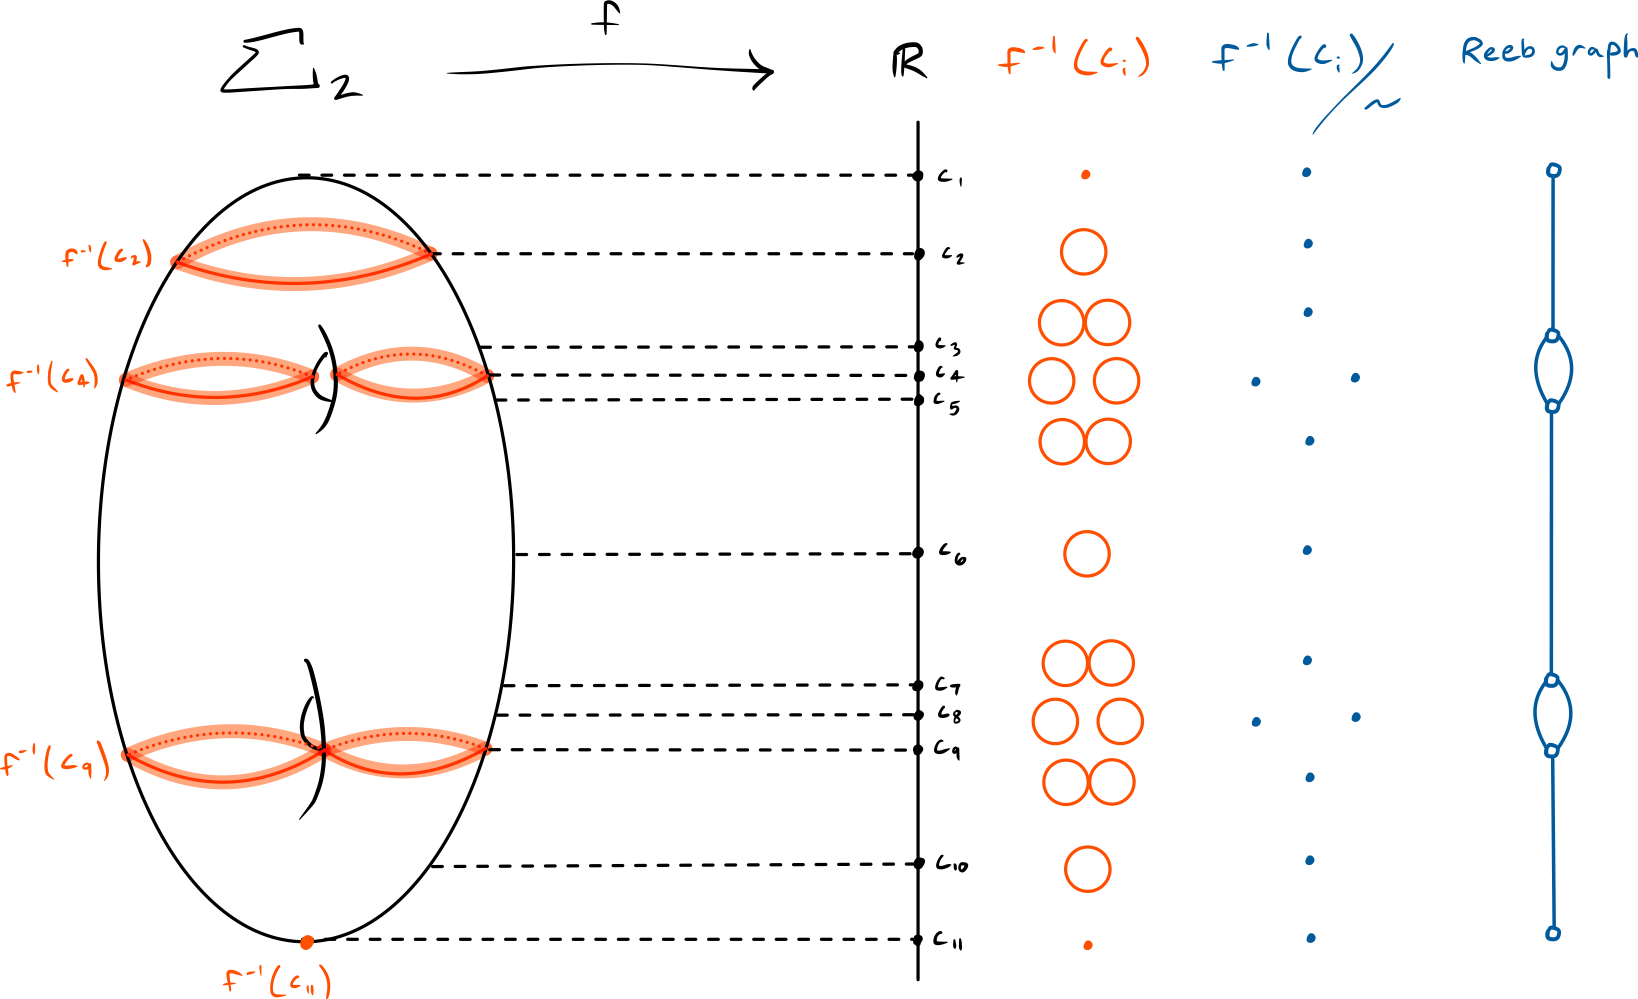
\includegraphics[width=1.1\textwidth]{reeb.png}
    \end{center}
  \end{figure}
\end{frame}

\begin{frame}{Mapper: Original Flavor}
\begin{itemize}
  \item How can we apply this to the discrete setting?
  \item Topological space $X \implies$ point cloud $P$ (a discrete set of points in a space)
  \item Filter function: $f: P\implies\mathbb{R}$
  \item Level sets of points $\implies$ level sets of overlapping intervals
  \item Connected components $\implies$ clusters
  \item Quotient space $\implies$ nerve complex
\end{itemize}
\end{frame}

\begin{frame}{Filtering}
  \begin{figure}
    \begin{center}
      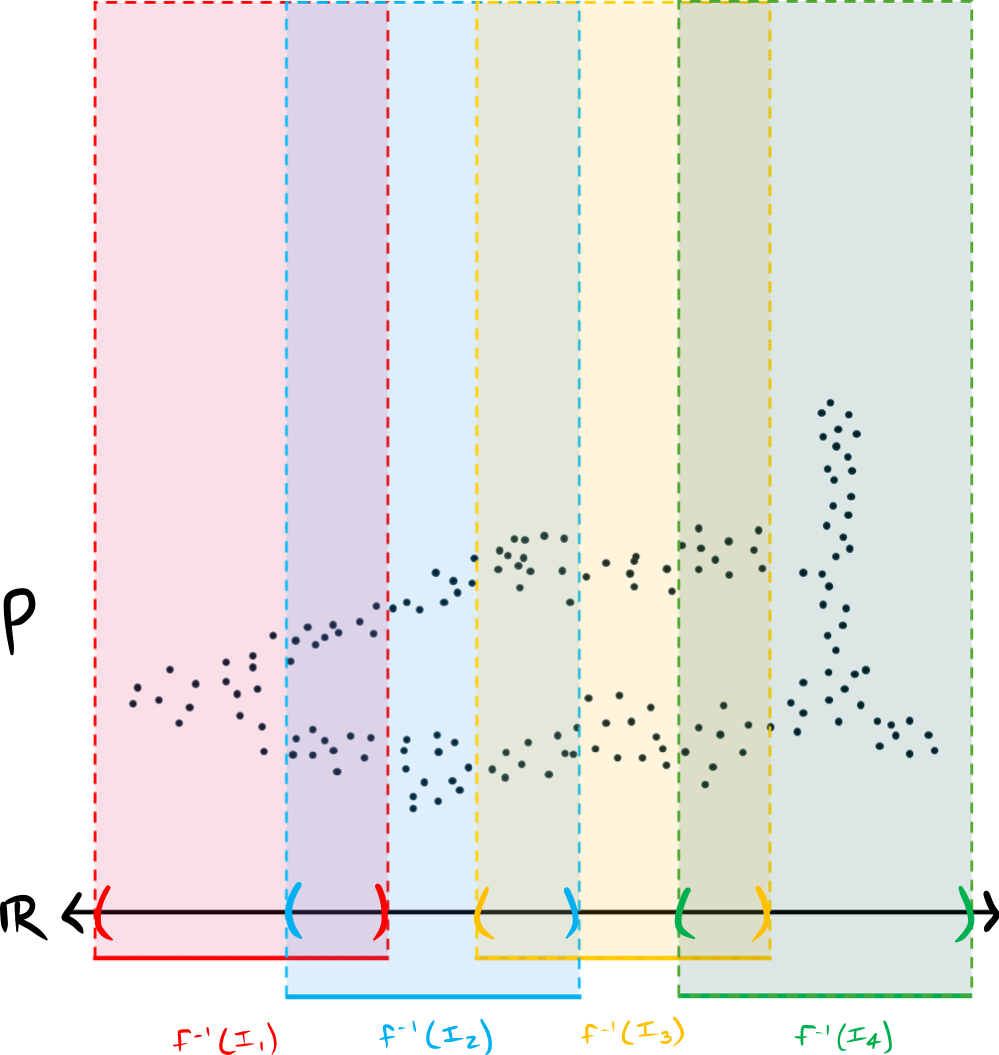
\includegraphics[width=.8\textwidth]{filteredposterdata.png}
    \end{center}
  \end{figure}
\end{frame}

\begin{frame}{Clustering}
  \begin{figure}
    \begin{center}
      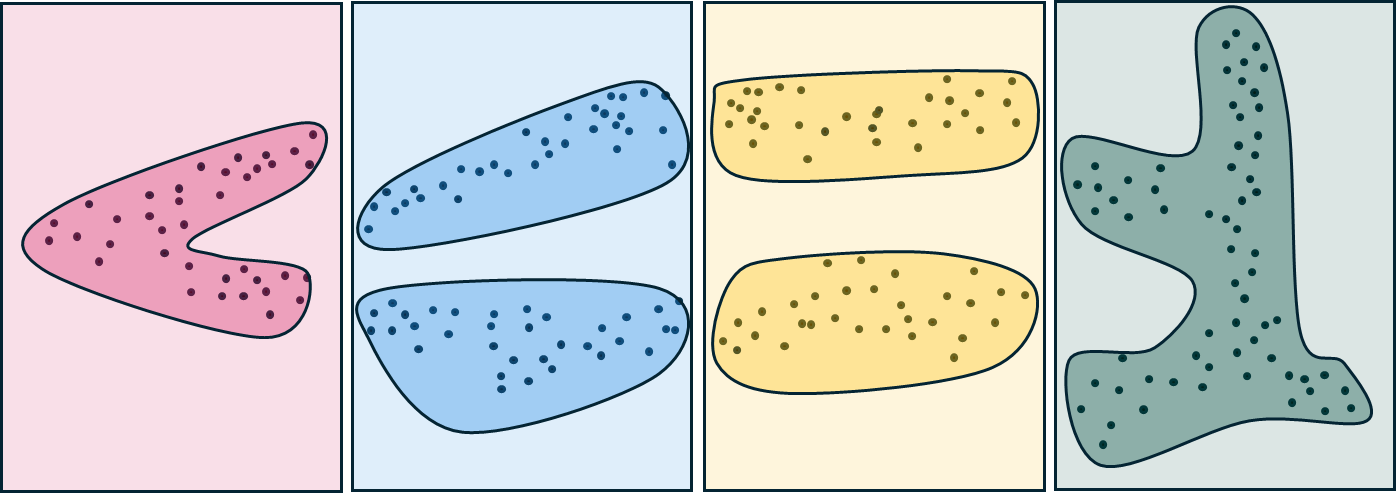
\includegraphics[width=1\textwidth]{posterdataclusters.png}
    \end{center}
  \end{figure}
\end{frame}

\begin{frame}{Nerve Construction}
  \begin{figure}
    \begin{center}
      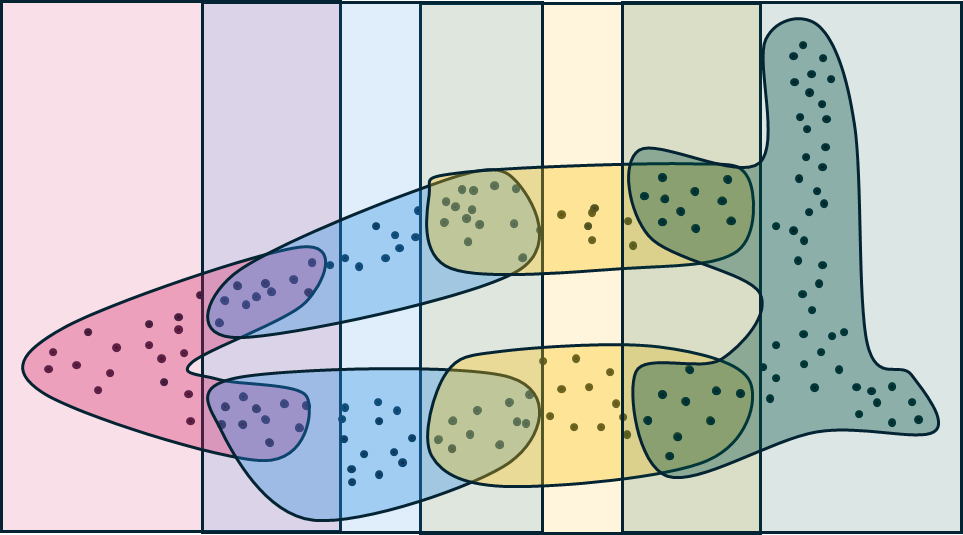
\includegraphics[width=.8\textwidth]{intersectposterdata.png}
    \end{center}
  \end{figure}
\end{frame}

\begin{frame}{Output}
  \begin{figure}
    \begin{center}
      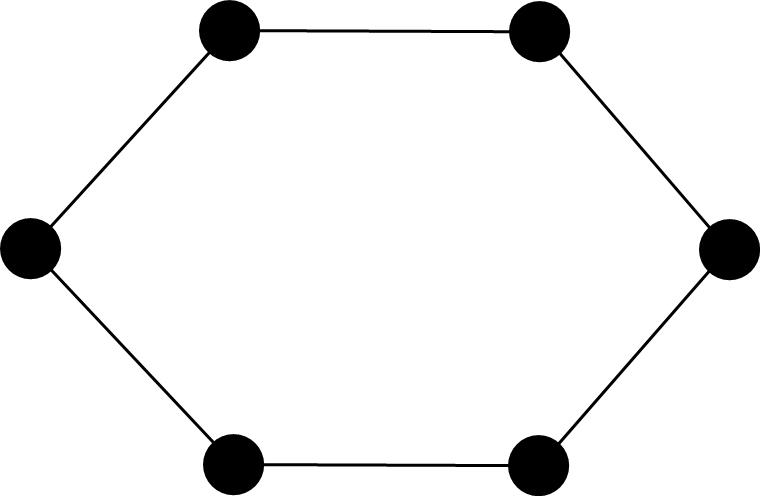
\includegraphics[width=.8\textwidth]{postermapper.png}
    \end{center}
  \end{figure}
\end{frame}

\begin{frame}{Ballmapper}
  \begin{itemize}
    \item Original flavor has a lot of choices to make
    \item Idea: come up with a one-parameter Mapper
    \item Ballmapper: in place of a conventional filter, cover the dataset with overlapping $\varepsilon$-balls
    \item Specifically, we want a cover $C = \bigcup_i B(x_i, \varepsilon)$ such that:
    \begin{itemize}
      \item Every datapoint $x$ is contained in some $B(x_i, \varepsilon)$ for some $x_i$
      \item If $x_j$ is a ball center, then the only ball containing it is $B(x_j, \varepsilon)$
    \end{itemize}
    \item Nerve construction is the same
  \end{itemize}
  
\end{frame}

\begin{frame}{Ballmapper: Cover}
  \begin{figure}
    \begin{center}
      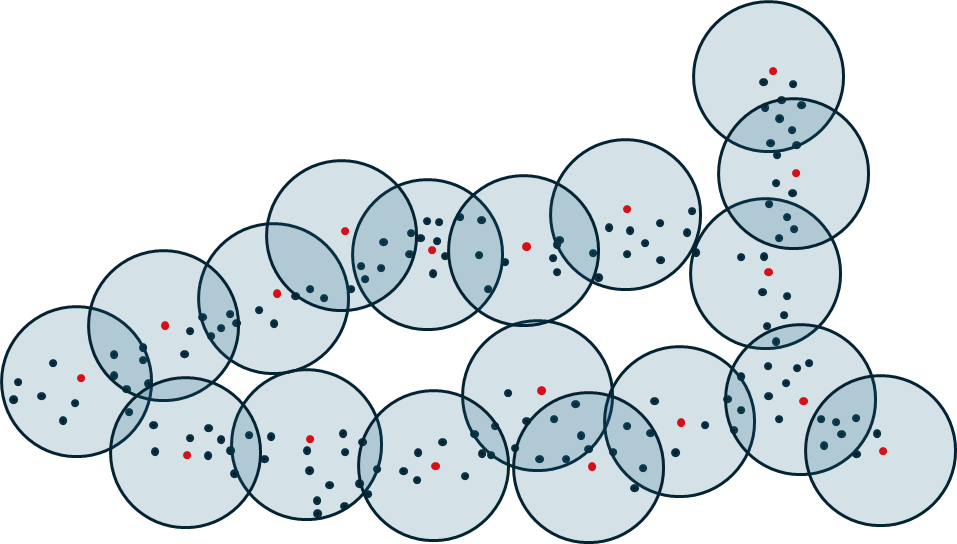
\includegraphics[width=1\textwidth]{ballcover.png}
    \end{center}
  \end{figure}

\end{frame}

\begin{frame}{Ballmapper: Nerve}
  \begin{figure}
    \begin{center}
      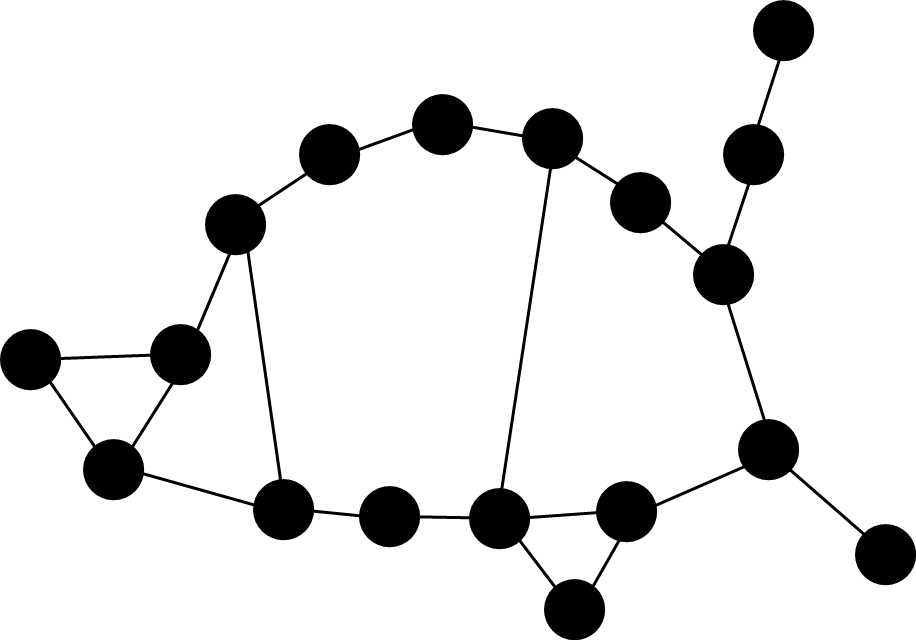
\includegraphics[width=1\textwidth]{ballmapperposter.png}
    \end{center}
  \end{figure}
\end{frame}

\begin{frame}{Refined Ballmapper}
  \begin{itemize}
    \item Idea: combine Ball filtering and Original clustering
    \item Bin by balling, then cluster within balls as in Original
    \item Output graph $R$ is a refinement of Ballmapper output $B$; there 
    is a natural graph homomorphism $\phi: R\to B$ which simply maps vertices into their balls
    \item Allows for comparison of two different metrics at the same time
  \end{itemize}
  
\end{frame}

\begin{frame}{Standard Ballmapper}
  \begin{figure}
    \begin{center}
      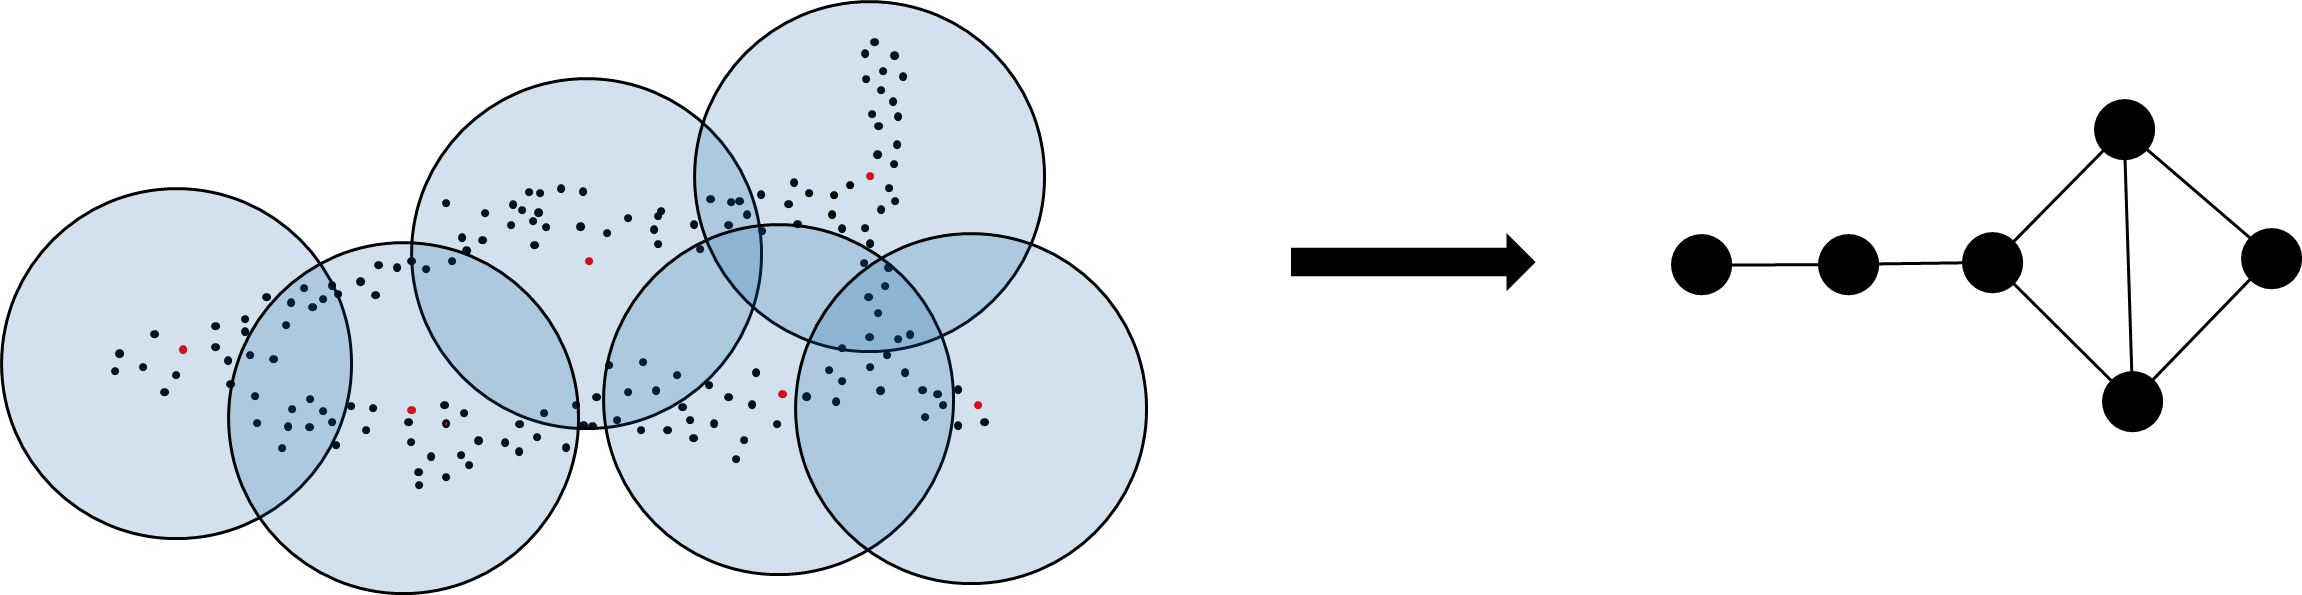
\includegraphics[width=1\textwidth]{prerefined.png}
    \end{center}
  \end{figure}
\end{frame}

\begin{frame}{Balls as Bins}
  \begin{figure}
    \begin{center}
      \hspace*{-.5cm}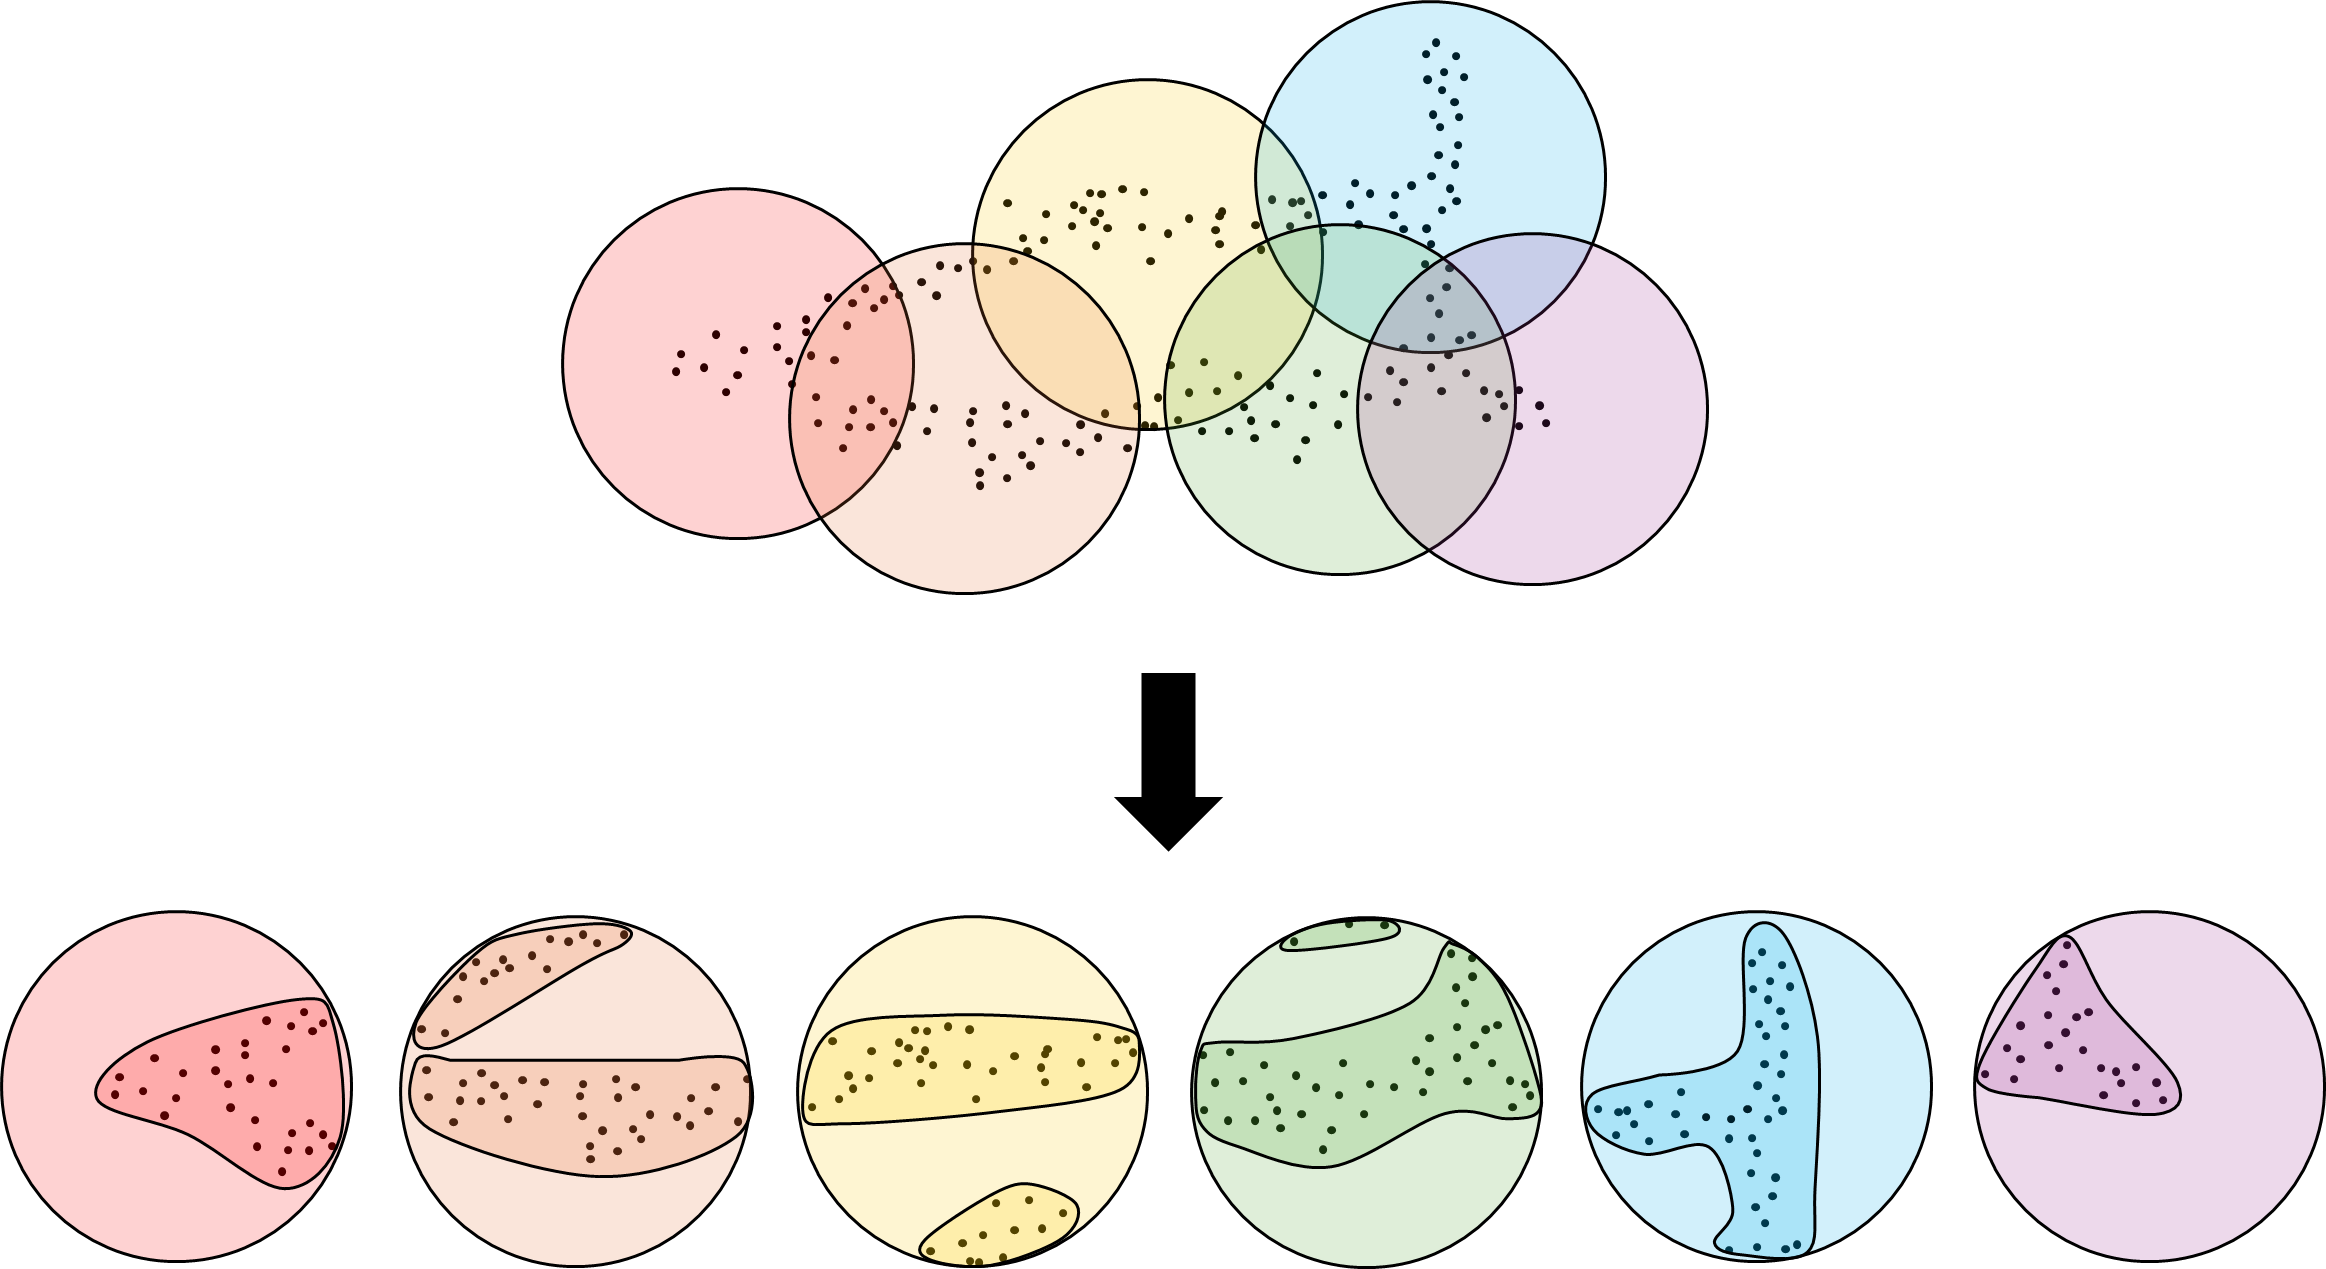
\includegraphics[width=1.1\textwidth]{ballclustering.png}
    \end{center}
  \end{figure}
\end{frame}

\begin{frame}{Refined Ballmapper Graph}
  \begin{figure}
    \begin{center}
      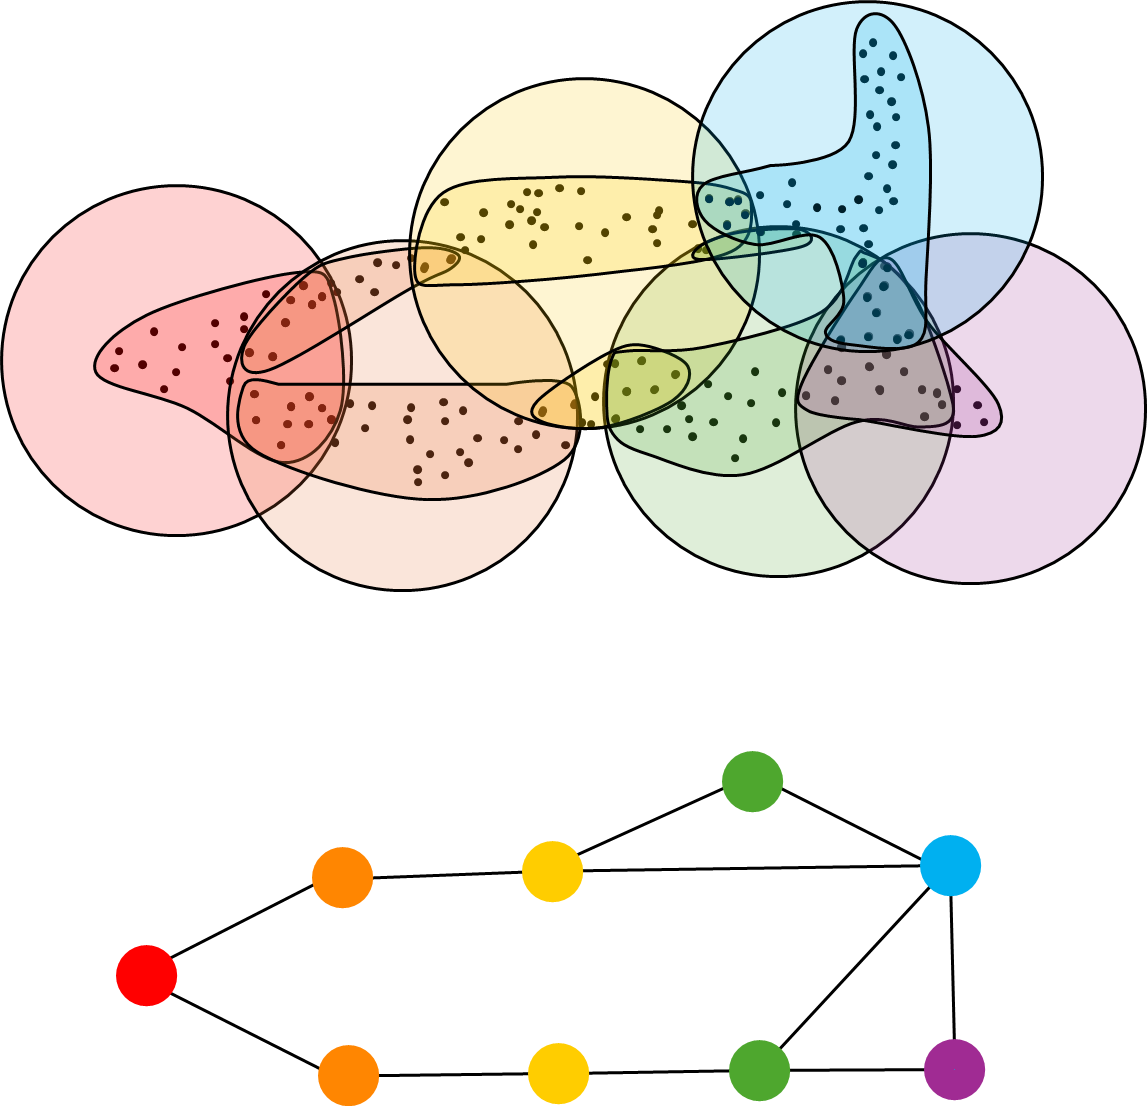
\includegraphics[width=.75\textwidth]{refinedballmapper.png}
    \end{center}
  \end{figure}
\end{frame}

\begin{frame}{Graph Theoretic Relation}
  \begin{itemize}
    \item A function $\phi$ between the vertices of two graphs $G$ and $H$ is called a \textbf{graph homomorphism} if $uv\in E(G)$ implies $\phi(uv)\in E(H)$.
    \item $G$ and $H$ are called \textbf{homomorphically equivalent} (hom-equivalent) if there exist graph homomorphisms $f: G\to H$ and $g: H\to G$.
  \end{itemize}
  \begin{figure}
    \begin{center}
      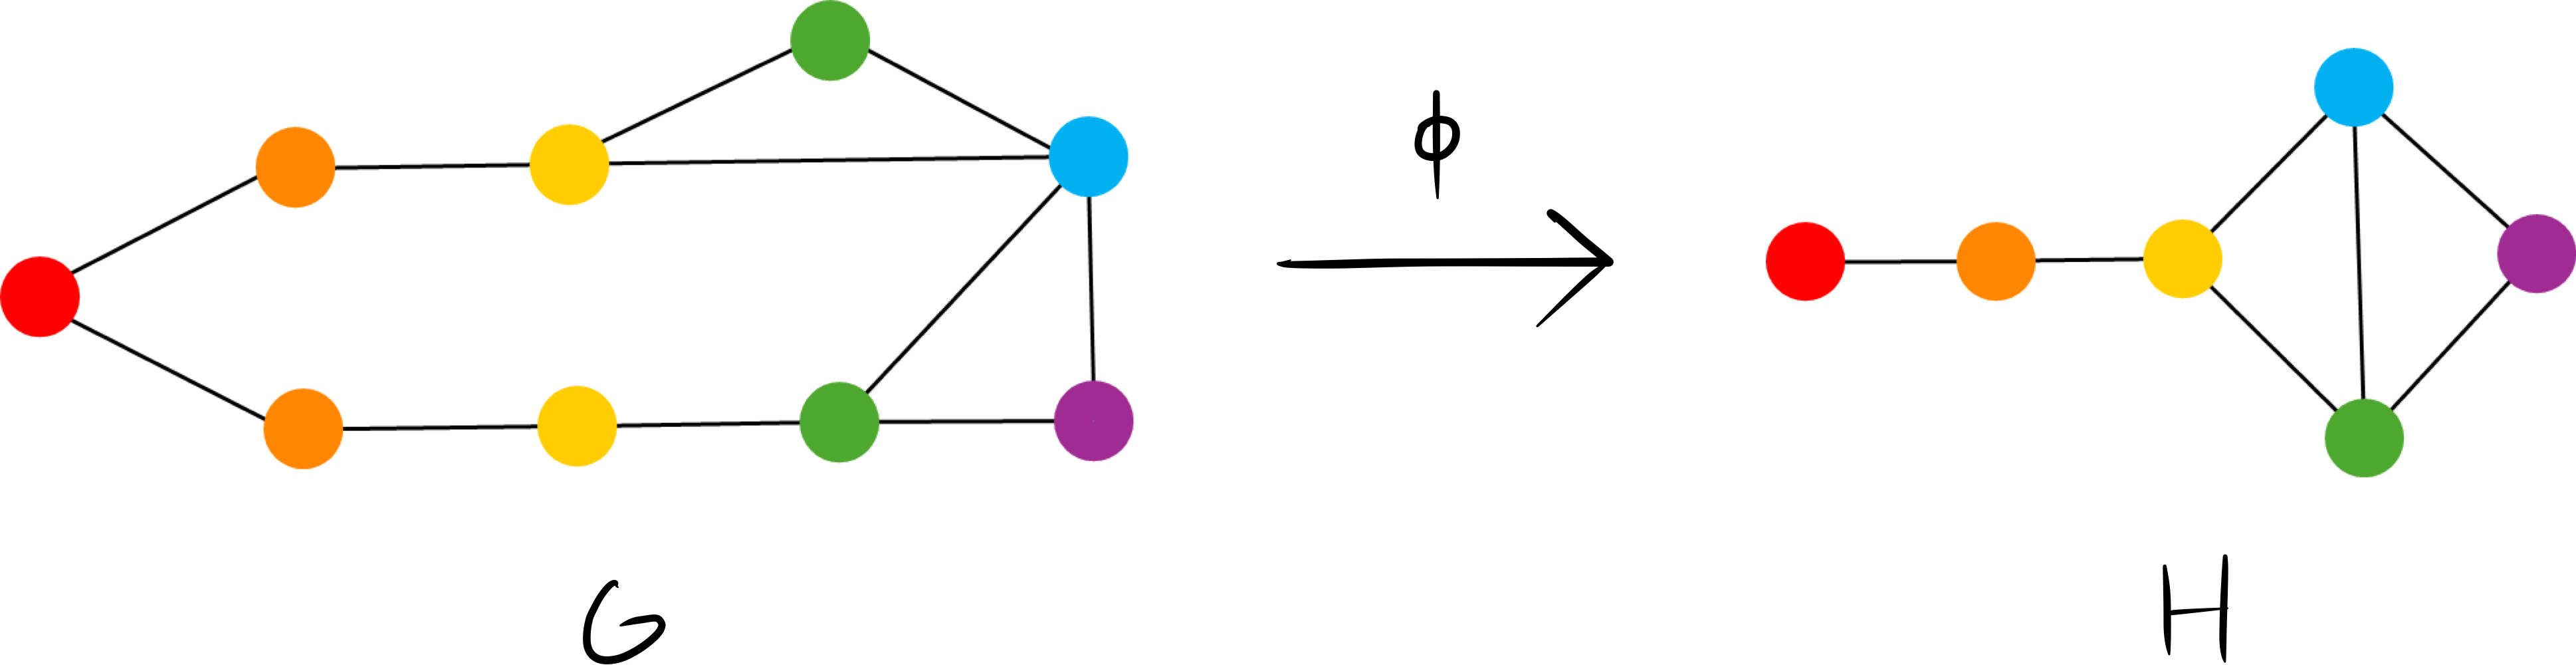
\includegraphics[width=1\textwidth]{graphhomo.png}
    \end{center}
  \end{figure}
\end{frame}

\begin{frame}{Why Might We Care? Possibility: Cores}
  \begin{itemize}
    \item A \textbf{core} $C$ of a graph $G$ is a graph such that $G$ and $C$ are hom-equivalent, and $C$ is the smallest such graph.
    \begin{itemize}
      \item Complete graphs, odd cycles, etc
    \end{itemize}
    \item Every finite graph has a core, and it is unique (up to isomorphism).
    \item Graphs with the same cores are necessarily hom-equivalent, and vice versa.
    \item Core-finding complexity: NP-complete :(
    \item Applications to relational algebra
  \end{itemize}
\end{frame}

\begin{frame}{Example Equivalence via Core}
  \begin{figure}
    \begin{center}\hspace*{-.3cm}
      \only<1>{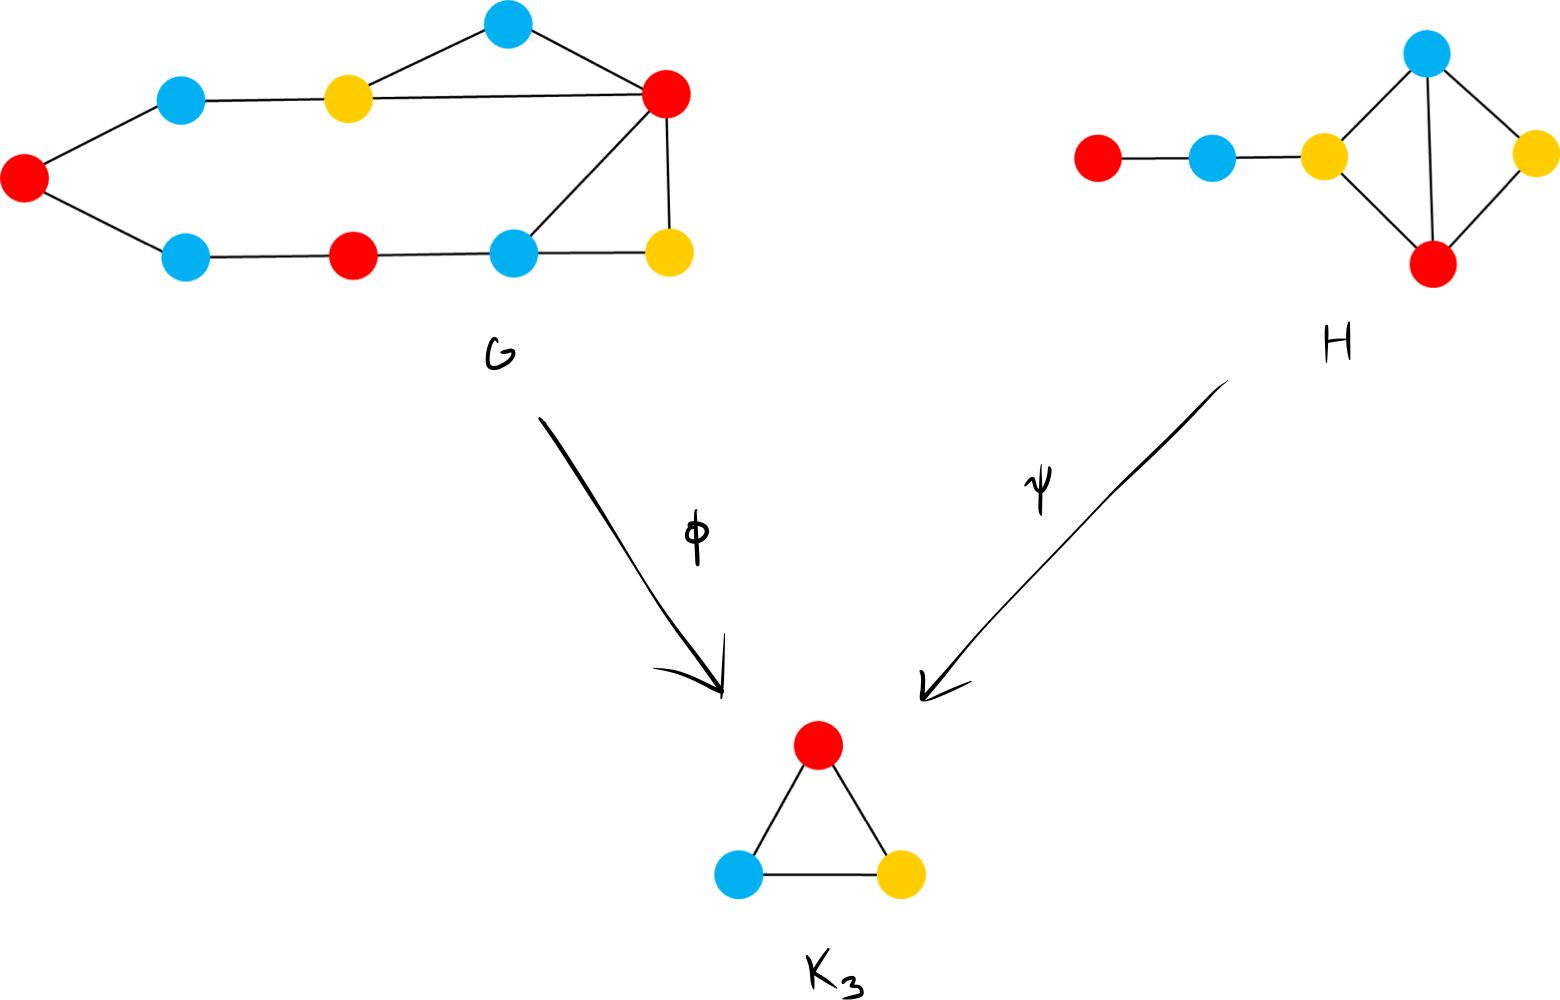
\includegraphics[width=1.05\textwidth]{graphcore.png}}
      \only<2>{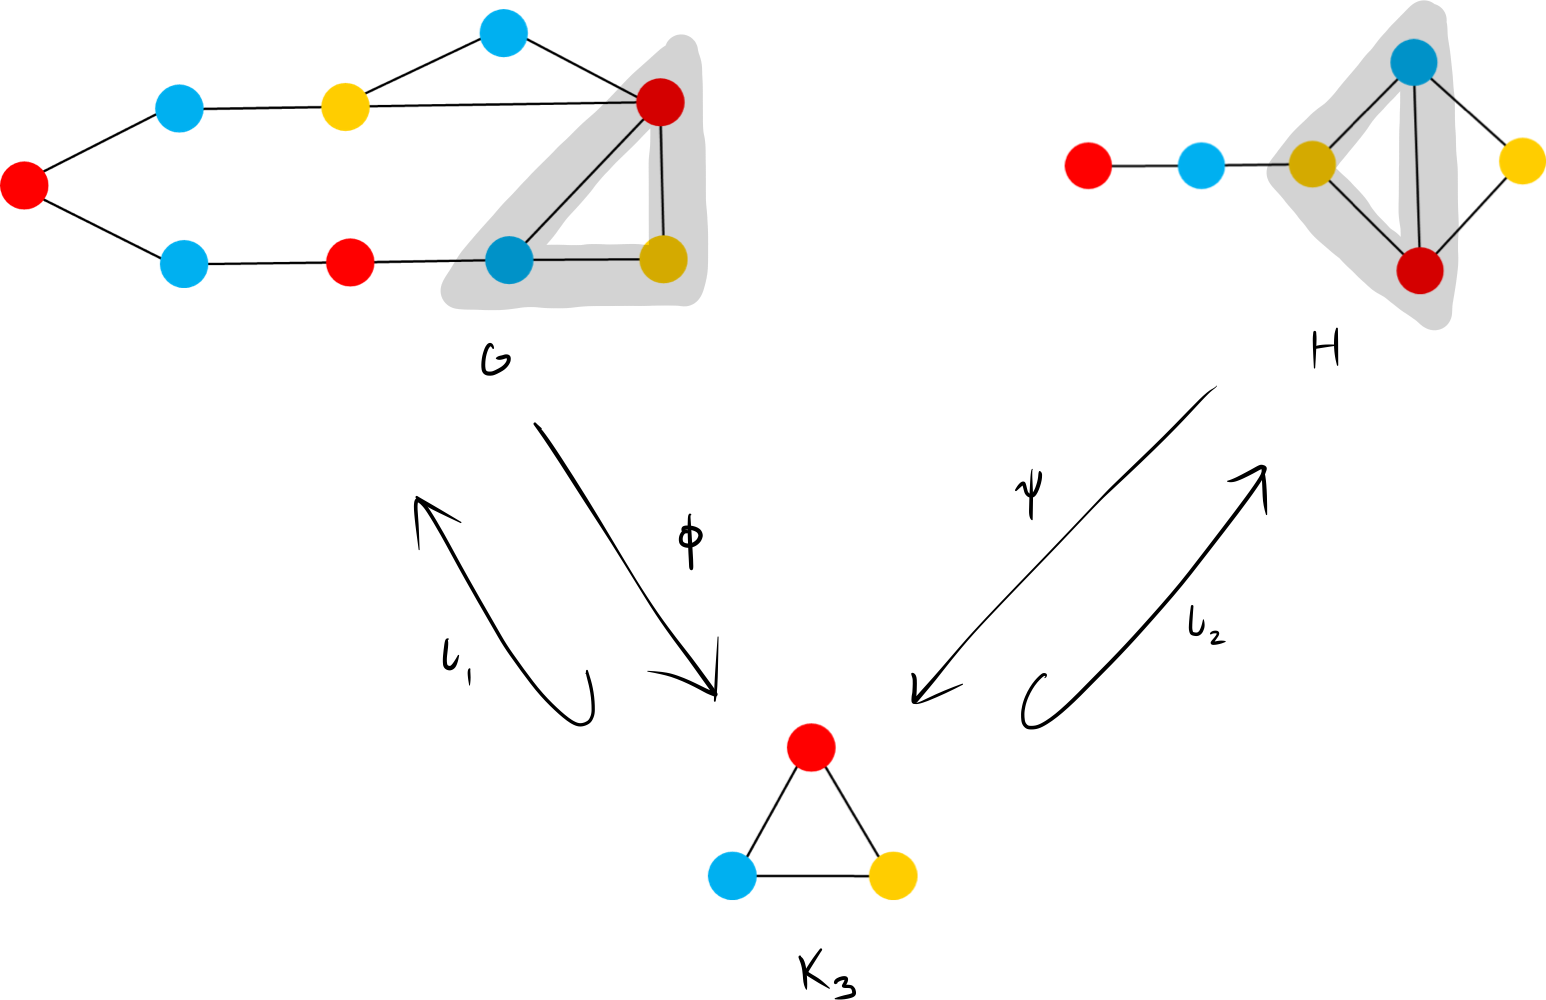
\includegraphics[width=1.05\textwidth]{graphcoreinclusion.png}}
    \end{center}
  \end{figure}
  \begin{figure}
    \begin{center}\vspace*{-1.65cm}\hspace*{-.3cm}
      \only<3>{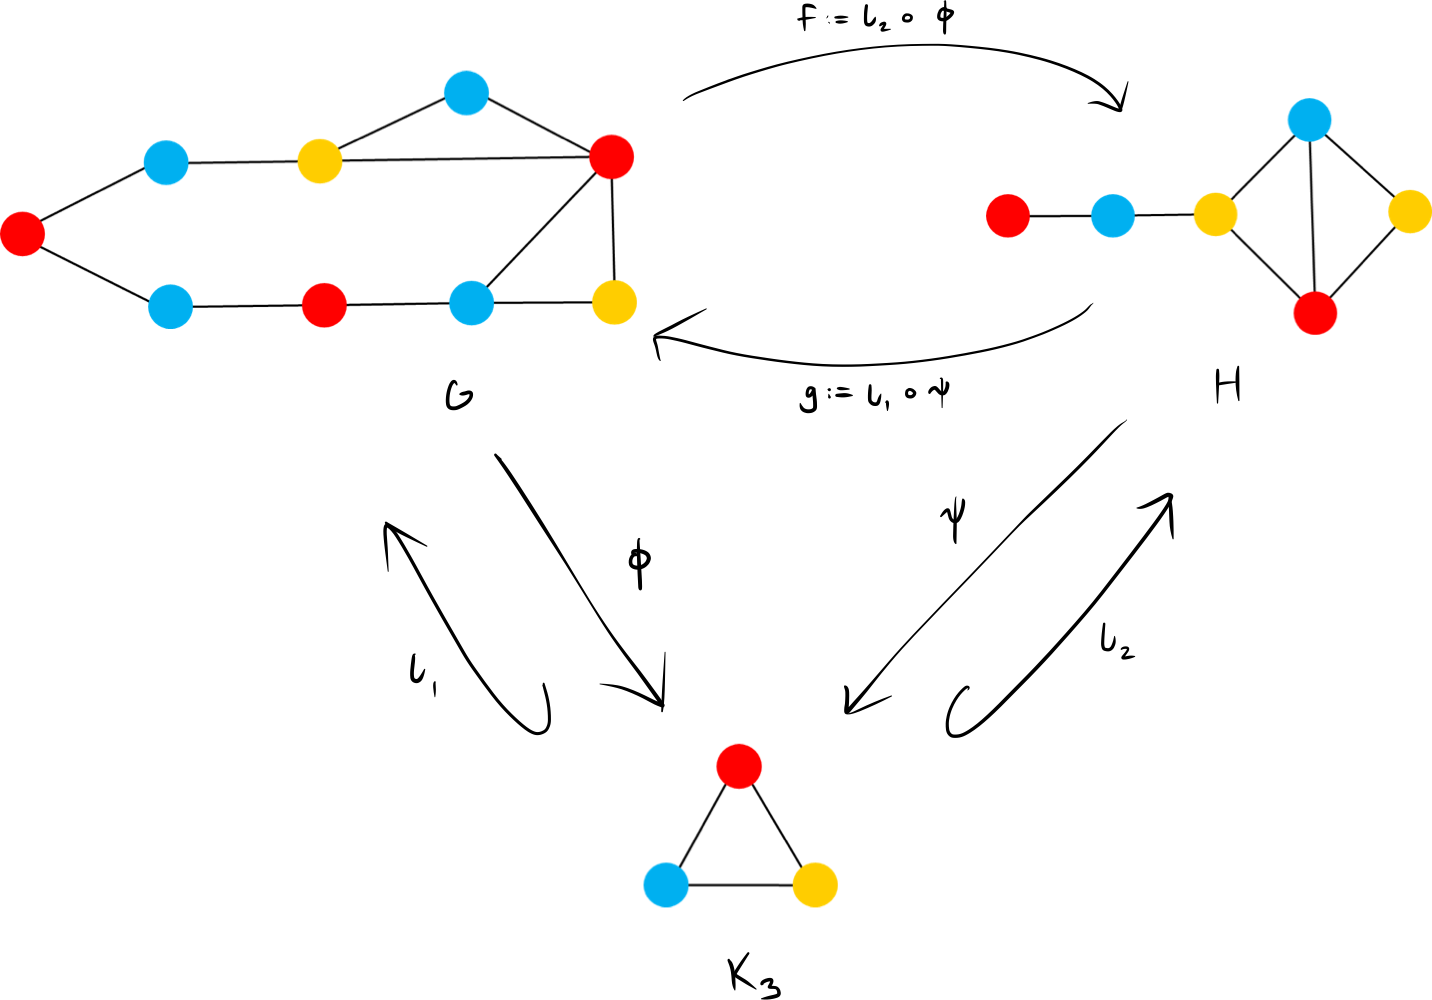
\includegraphics[width=1.05\textwidth]{graphcorefull.png}}
    \end{center}
  \end{figure}
\end{frame}

\begin{frame}{Problems}
  \begin{itemize}
    \item We lost so much stuff! That clustering took work...
    \item Graphs are abstract combinatorial structures; they convey no geometrical information
    \item Potentially interesting features can ``bypass'' the filter
    \item Output heavily depends on your choices of parameters and clustering method
  \end{itemize}
  
\end{frame}
\section{Cytoscape to the Rescue}
\begin{frame}{What is Cytoscape?}
  \begin{itemize}
    \item Powerful network analysis software (written in Java)
    \item Used primarily by bioinformaticists but is a general use program
  \end{itemize}
  \begin{figure}
    \begin{center}
      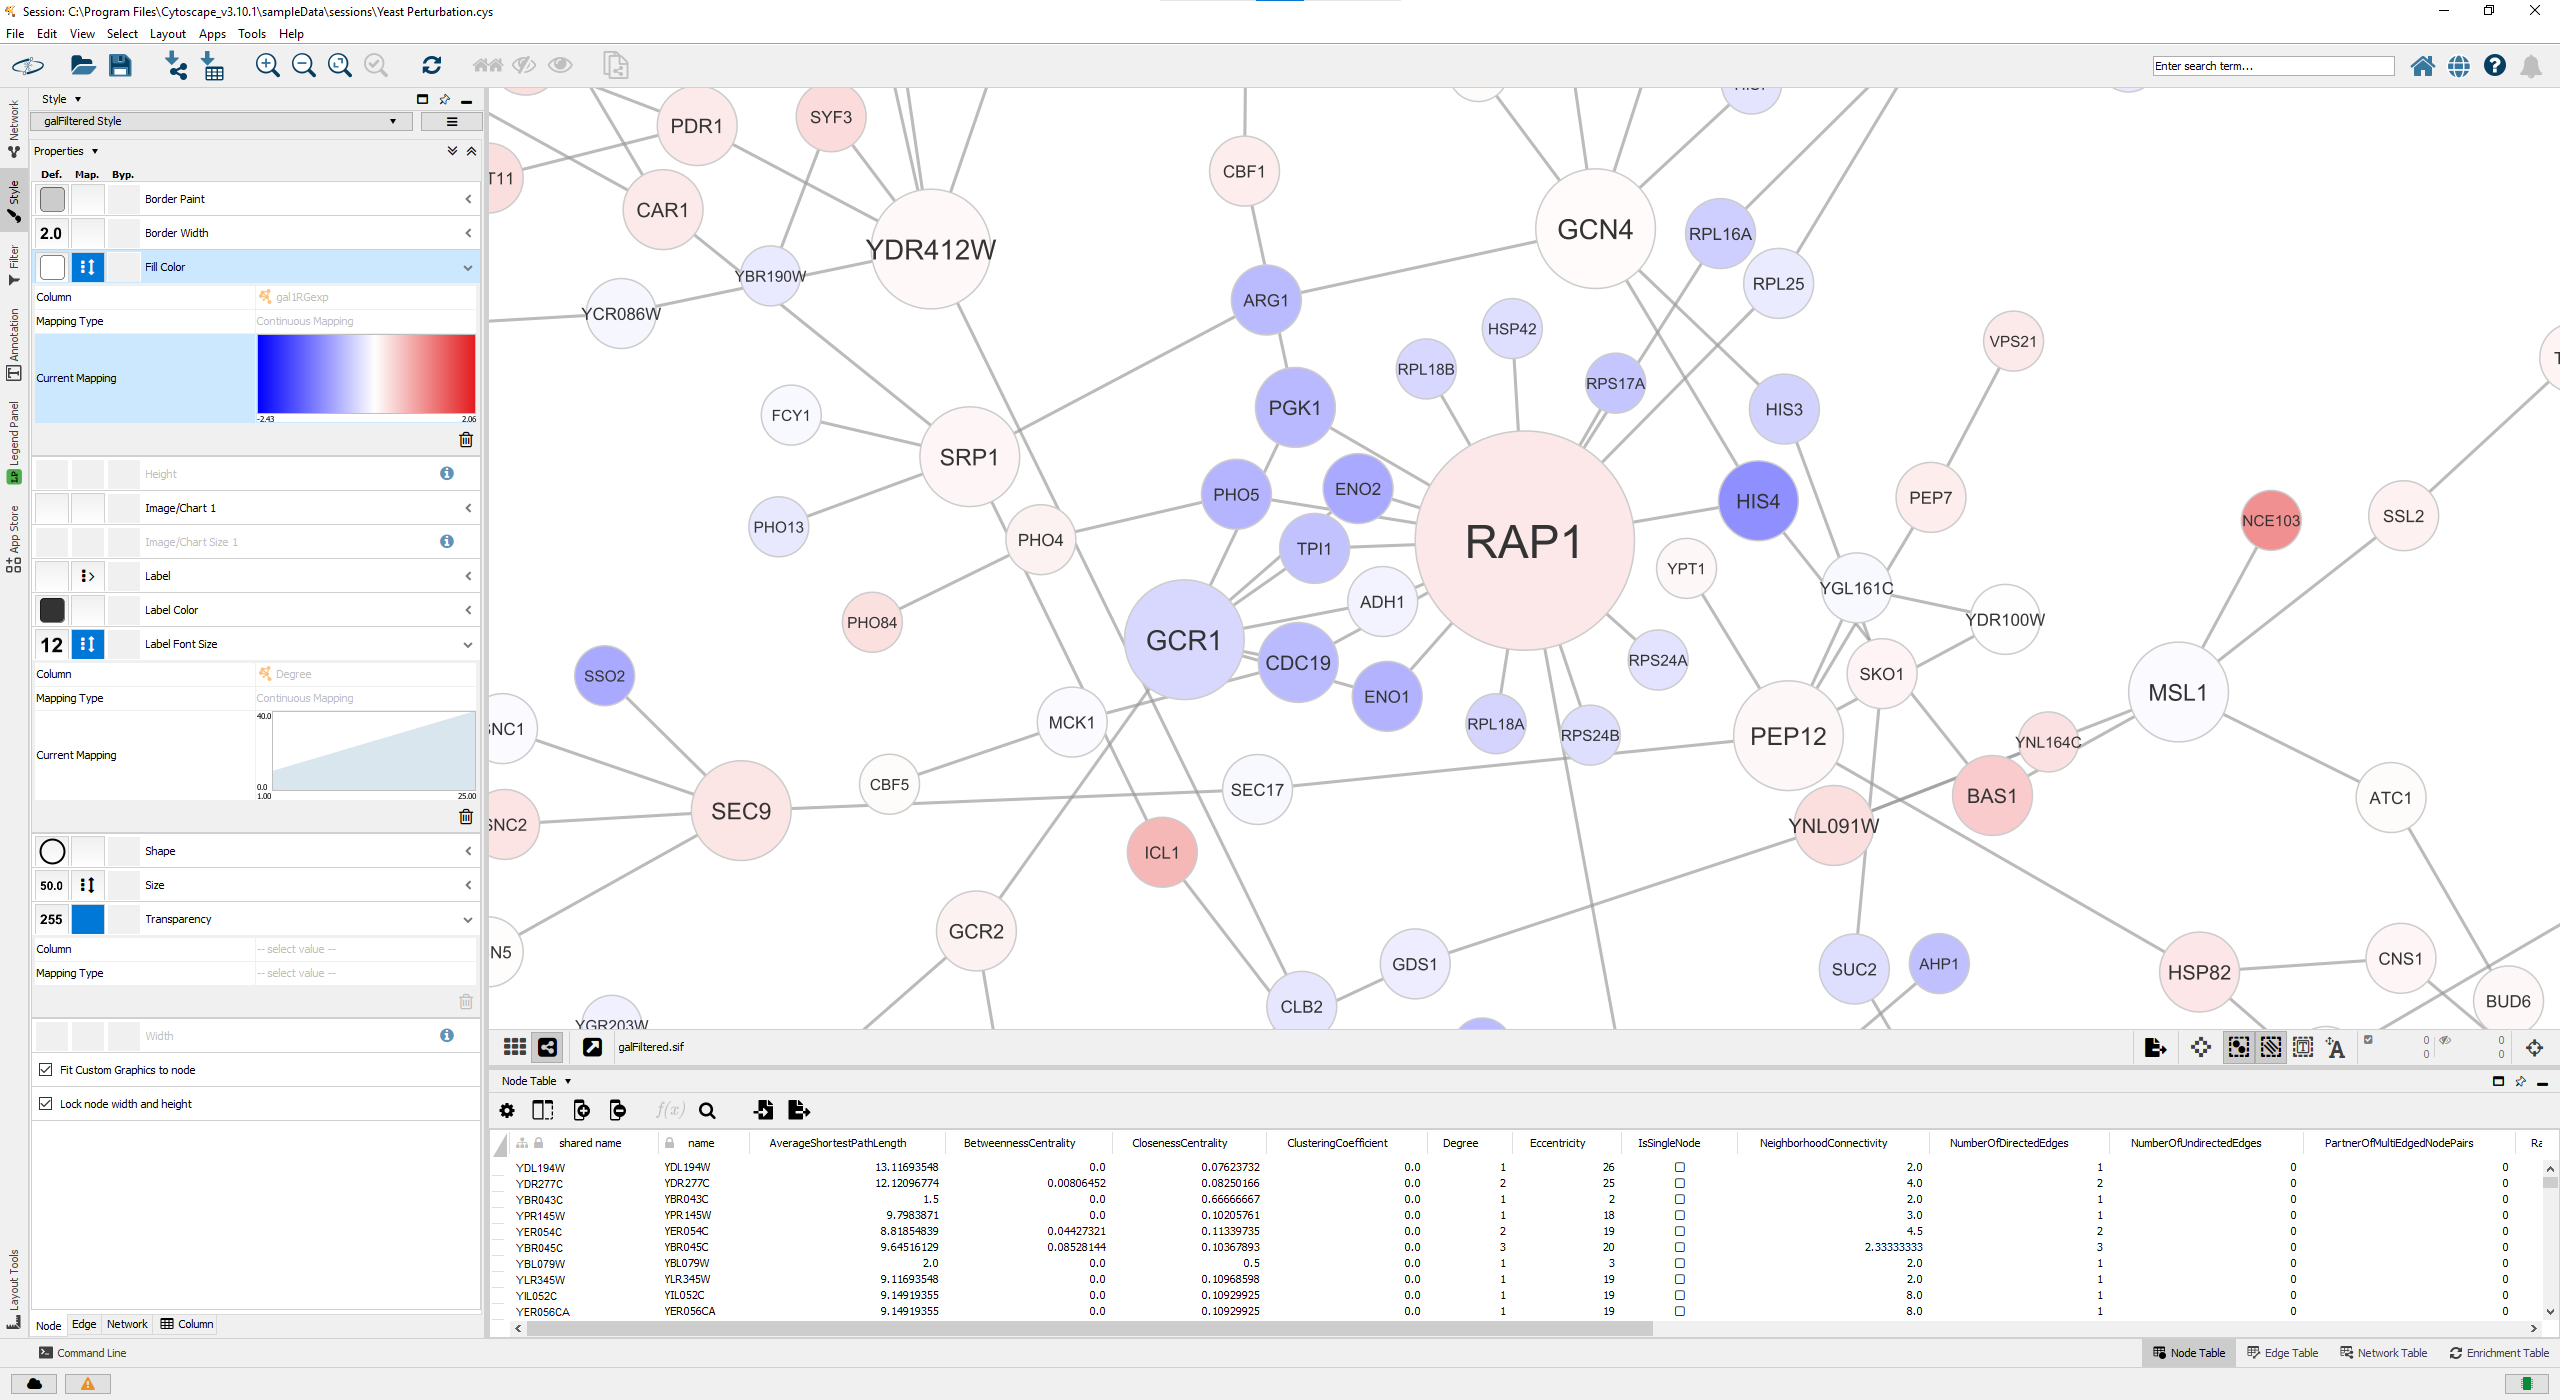
\includegraphics[width=1\textwidth]{cytoyeast.png}
    \end{center}
  \end{figure}
\end{frame}

\begin{frame}{Features}
  \begin{itemize}
    \item Networks are stored as separate tables of nodes and edges
    \item Tables can be augmented with any number or type of columns
    \item Any column can then be associated with a visual characteristic of the network
  \end{itemize}
  \begin{figure}
    \begin{center}
      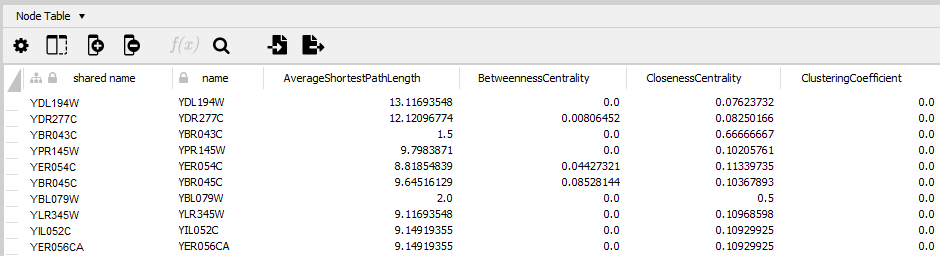
\includegraphics[width=1\textwidth]{nodetable.png}
    \end{center}
  \end{figure}
\end{frame}

\begin{frame}{Styling Mapper: Vertices}
  \begin{itemize}
    \item Node size/label $\to$ cluster size
    \item Node border color $\to$ associated level set/filter value/ball
    \item Node fill color $\to$ cluster dispersion
  \end{itemize}
  \begin{figure}
    \begin{center}
      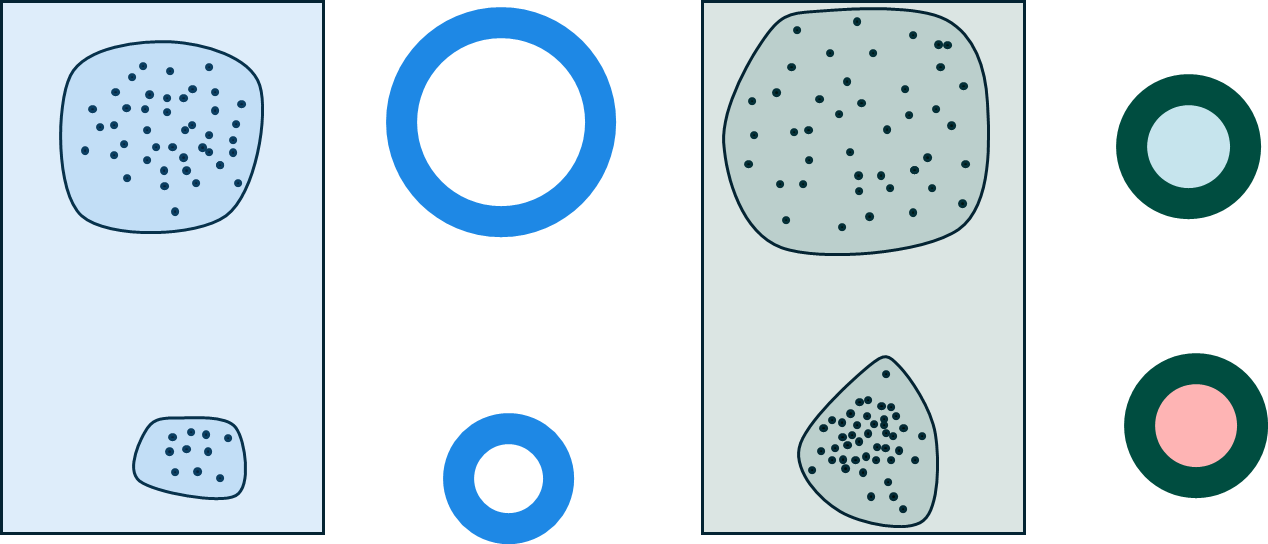
\includegraphics[width=1\textwidth]{nodestyling.png}
    \end{center}
  \end{figure}
\end{frame}

\begin{frame}{Styling Mapper: Edges}
  \begin{itemize}
    \item Edge thickness/opacity $\to$ cluster intersection strength
    \item Edge label $\to$ cluster intersection size
  \end{itemize}
  \begin{figure}
    \begin{center}
      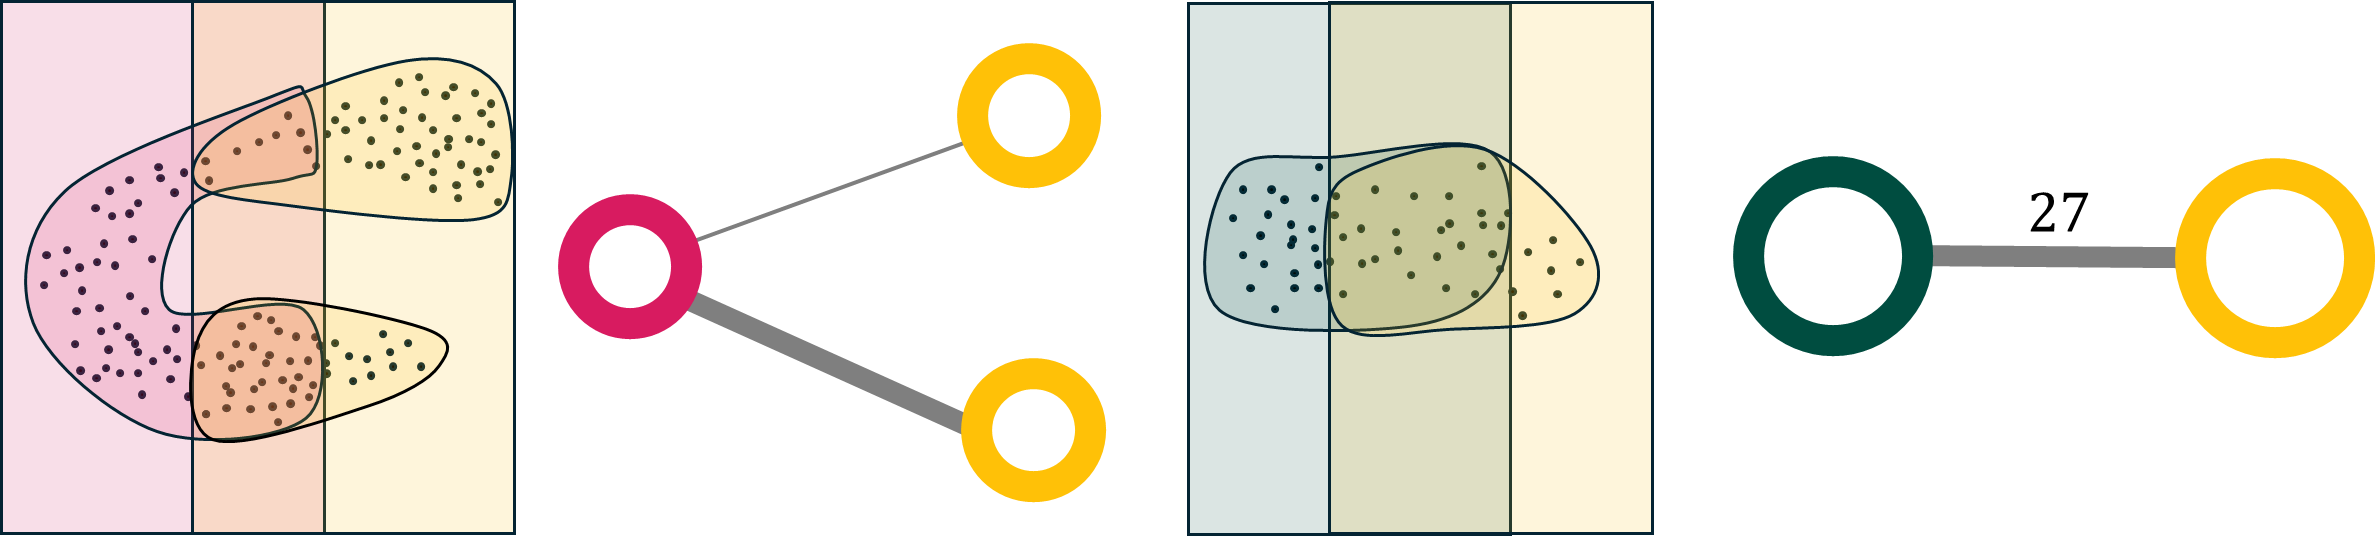
\includegraphics[width=1.05\textwidth]{edgestyling.png}
    \end{center}
  \end{figure}
\end{frame}

\begin{frame}{Exploring the Graph}
  \begin{itemize}
    \item Cytoscape can calculate classical network statistics
    \begin{itemize}
      \item Centrality measures
      \item Clustering coefficients
      \item Modularity classes
    \end{itemize}
    \item We can filter out nodes/edges by characteristics
  \end{itemize}
  \begin{figure}
    \begin{center}
      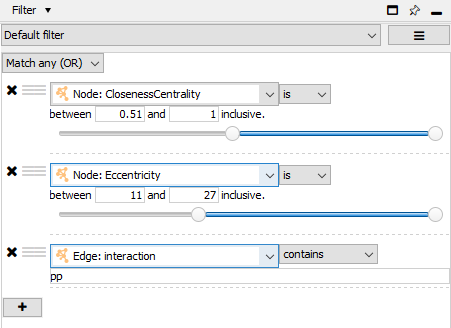
\includegraphics[width=.65\textwidth]{cytofilter.png}
    \end{center}
  \end{figure}
\end{frame}

\begin{frame}{Possible Capabilities}
  \begin{itemize}
    \item Cytoscape is open source and was designed to be modified
    \item Possible projects here include:
    \begin{itemize}
      \item Assign energy function to edges and apply layout algorithm
      \item Animation between networks (say, from RBM to BM or reverse)
      \item More graph algorithms (finding cores, clique detection, etc)
    \end{itemize}
  \end{itemize}
  
\end{frame}
\section{Aptamers}
\begin{frame}{Biology CliffNotes CliffNotes}
  \begin{itemize}
    \item RNA (ribonucleic acid) and DNA (deoxyribonucleic acid) are polymers which carry genetic sequences and have additional structure
  \end{itemize}
  \begin{figure}
    \begin{center}
      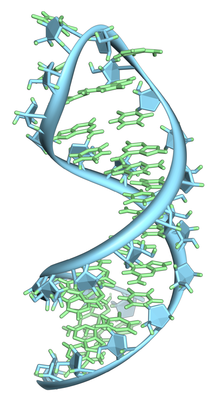
\includegraphics[width=.3\textwidth]{rna.png}
    \end{center}
  \end{figure}
\end{frame}

\begin{frame}{RNA and DNA}
  \begin{figure}
    \begin{center}
      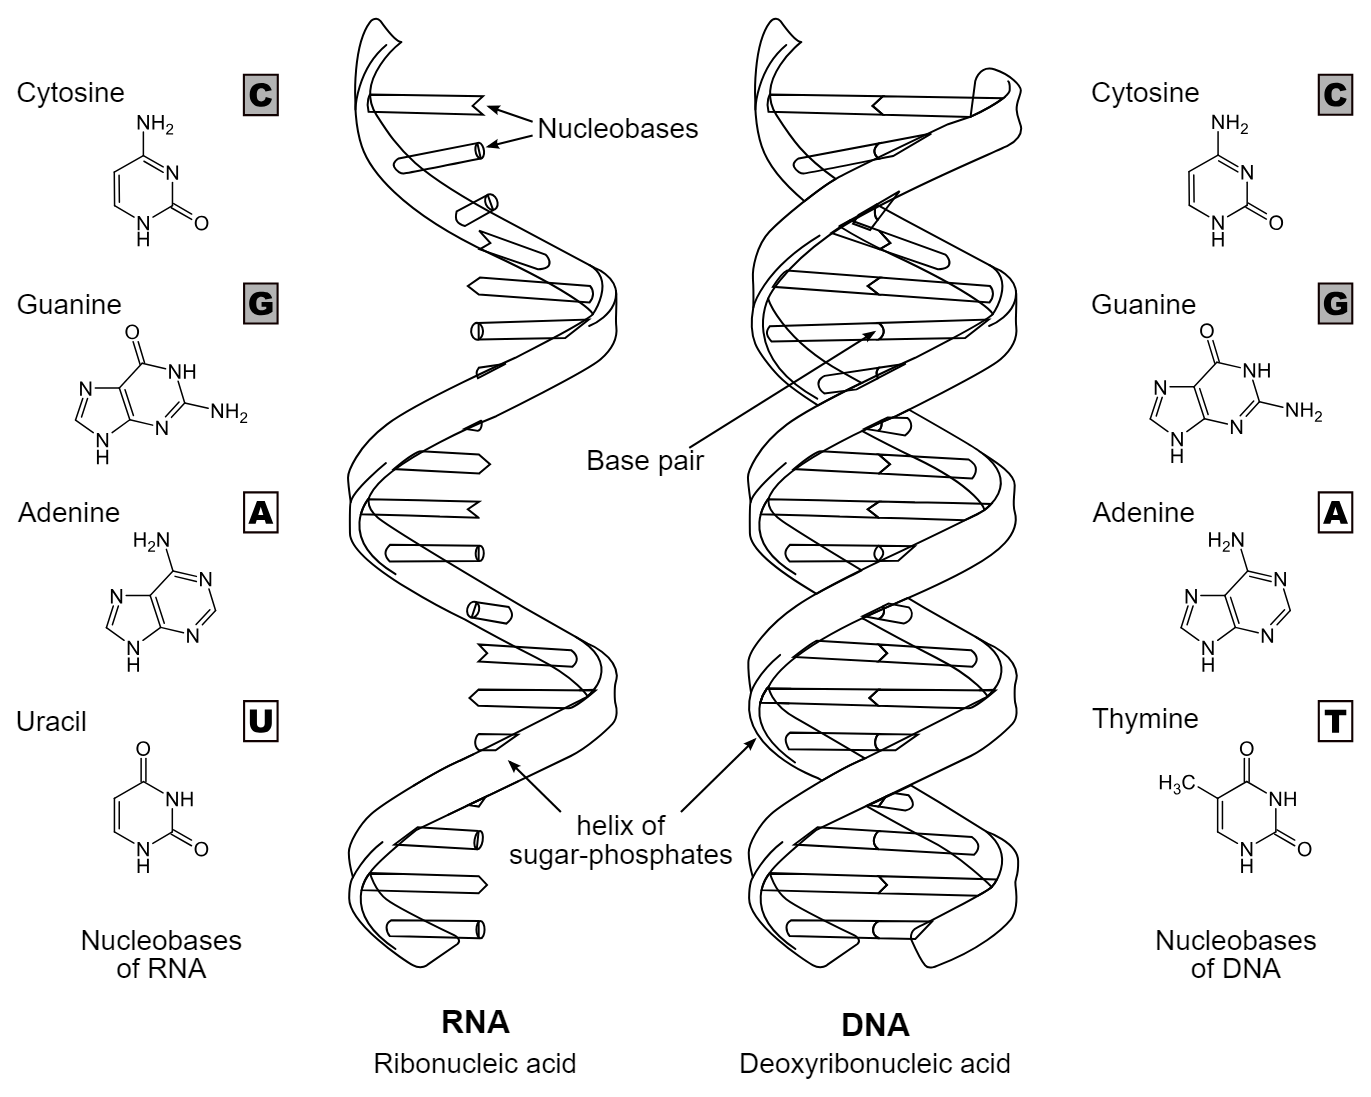
\includegraphics[width=1\textwidth]{rnadna.png}
    \end{center}
  \end{figure}
\end{frame}

\begin{frame}{What Is an Aptamer?}
\begin{itemize}
  \item Aptamers are synthetic RNA molecules that bind to a specific target
  \item Similar function to antibodies, but much smaller
  \item \textbf{Genetic code not expressed}
  \begin{figure}
    \begin{center}
      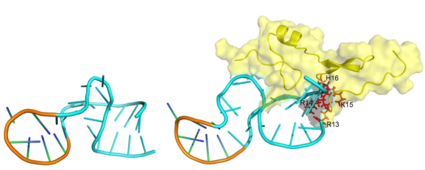
\includegraphics[width=1\textwidth]{aptamer.png}
    \end{center}  
  \end{figure}
\end{itemize}
  
\end{frame}

\begin{frame}{Comparing Aptamers}
  \begin{itemize}
    \item For TDA to work we need a metric\footnote{ehhhh...} by which to compare aptamers
    \item Aptamers have two characteristics: their genetic code and their structure
    \item Distance between sequences: Levenshtein distance
    \item Distance between structures: tree distance
  \end{itemize}
\end{frame}

\begin{frame}{Aptamer Metrics}
  \begin{figure}
    \begin{center}
      \hspace*{-.75cm}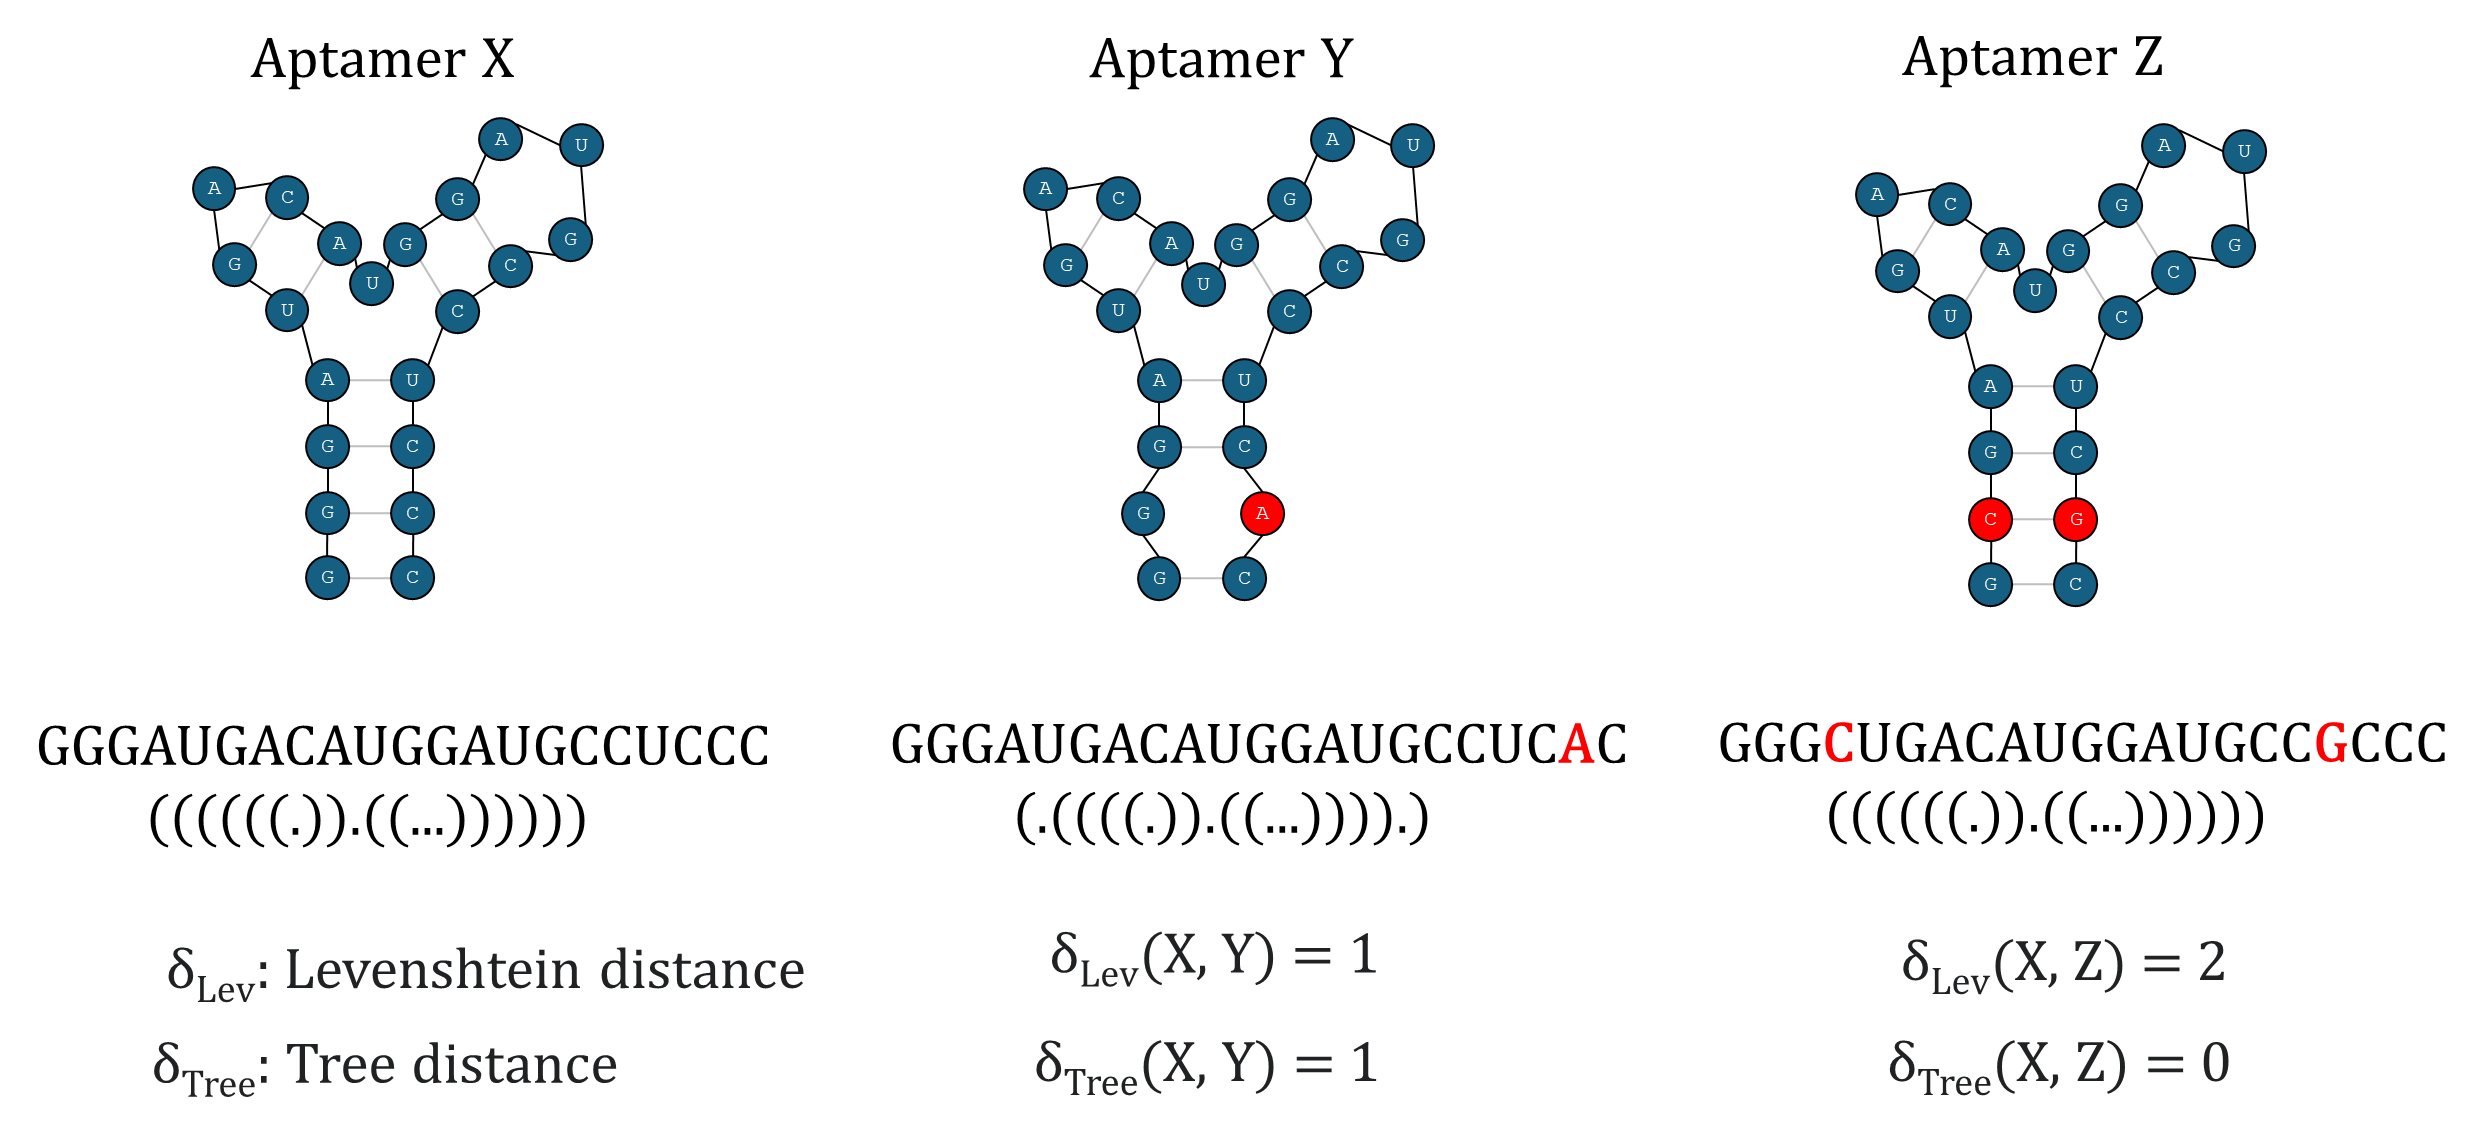
\includegraphics[width=1.15\textwidth]{aptamers.png}
    \end{center}
  \end{figure}
\end{frame}

\begin{frame}{Aptamer Clustering With Mapper}
  \begin{itemize}
    \item Flavor: Refined Ballmapper
    \item Idea: Ball using tree distance, cluster using Levenshtein distance
    \item Clustering method: single linkage hierarchical
    \item Vertices of the graph are clusters of aptamers related in both sequence and structure
    \item Graph structure may highlight families of aptamers or reveal other insights
  \end{itemize}
\end{frame}

\begin{frame}{Big Mapptamer Graph}
  \begin{figure}
    \begin{center}
      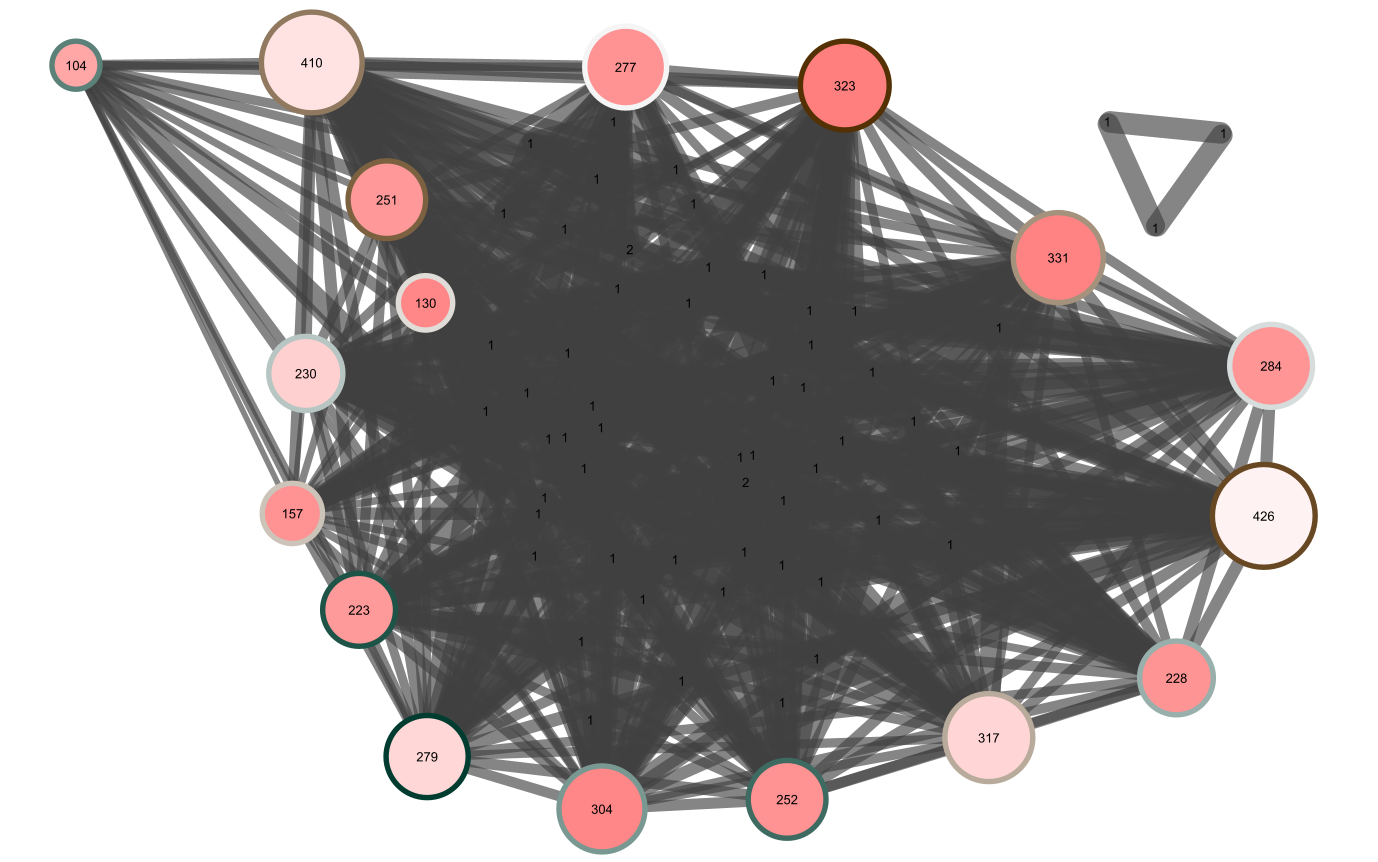
\includegraphics[width=1\textwidth]{bigmapptamer.png}
    \end{center}
  \end{figure}
\end{frame}

\begin{frame}{Pruned Mapptamer Graph}
  \begin{figure}
    \begin{center}
      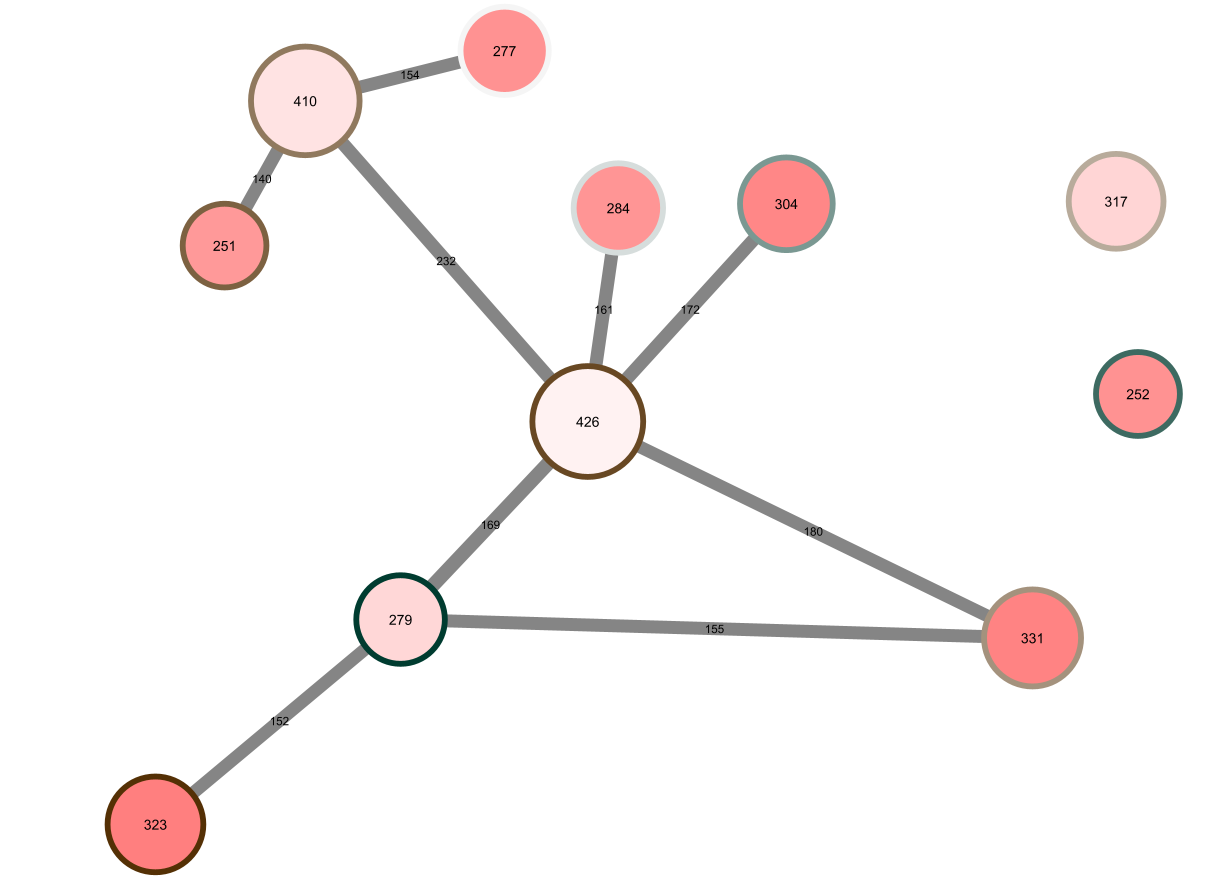
\includegraphics[width=1\textwidth]{prunedmapptamer.png}
    \end{center}
  \end{figure}
\end{frame}

\section{Mapping out Future Directions}
\subsection{Math}
\begin{frame}{Clustering}
  \begin{itemize}
    \item 
  \end{itemize}
\end{frame}

\begin{frame}{Stability}
  
\end{frame}

\begin{frame}{Persistence}
  
\end{frame}

\begin{frame}{Return of Reeb}
  
\end{frame}

\subsection{Biology}
\begin{frame}{More Aptamers}
  
\end{frame}

\begin{frame}{Neuroscience}

\end{frame}
\end{document}